\documentclass[conference]{IEEEtran}
\IEEEoverridecommandlockouts

% ── Packages ──────────────────────────────────────────────────────────────
\usepackage{cite}
\usepackage{array}
\usepackage{amsmath,amssymb,amsfonts}
\usepackage{algorithmic}
\usepackage{algorithm}
\usepackage{graphicx}
\usepackage{textcomp}
\usepackage{xcolor}
\usepackage{booktabs}
\usepackage{multirow}
\usepackage{url}
\usepackage{hyperref}
% \usepackage{balance}
\usepackage{microtype}

% ── Metadata ──────────────────────────────────────────────────────────────
\def\BibTeX{{\rm B\kern-.05em{\sc i\kern-.025em b}\kern-.08em
    T\kern-.1667em\lower.7ex\hbox{E}\kern-.125emX}}

\begin{document}

% ── Title ──────────────────────────────────────────────────────────────────
\title{ConceptGrade: A Knowledge Graph–Driven Framework for\\
       Concept-Aware Automated Short Answer Grading in\\
       Computer Science Education}

\author{
  \IEEEauthorblockN{Brahmaji Katragadda}
  \IEEEauthorblockA{
    \textit{Department of Computer Science} \\
    \textit{ICFAI (IFHE)} \\
    Hyderabad, India \\
    kbrahmaji.scholar25@ifheindia.org
  }
  \and
  \IEEEauthorblockN{Dr. P. Pavan Kumar}
  \IEEEauthorblockA{
    \textit{Department of Computer Science} \\
    \textit{ICFAI (IFHE)} \\
    Hyderabad, India
  }
}

\maketitle

% ── Abstract ───────────────────────────────────────────────────────────────
\begin{abstract}
How well does a hybrid Knowledge-Graph + Large Language Model (KG-LLM)
system actually work for Automated Short Answer Grading (ASAG) in
Computer Science education, and where does it stop working? We present
\textbf{ConceptGrade}, a five-layer framework that converts each
student answer into a \emph{concept graph} and compares it against an
expert-built Data Structures knowledge graph (101 concepts, 138 typed
relationships). We test it on $n = 2{,}276$ graded answers across 213
questions from three independent datasets (Mohler 2011, DigiKlausur,
Kaggle ASAG), against a zero-shot LLM baseline that uses the identical
underlying model. On its best dataset, ConceptGrade lowers error by
$8.2\%$ (Mohler 2011), though the gain is only marginally significant
once question non-independence is accounted for. DigiKlausur shows a
smaller but real gain. Kaggle ASAG shows none: its vocabulary falls
entirely outside the knowledge graph. A real-data ablation tells us why
the headline number is so modest in the first place -- the
deterministic knowledge-graph score, on its own, is $86.9\%$
\emph{worse} than the zero-shot baseline. Almost all of ConceptGrade's
net gain turns out to come from its LLM verifier stage, not the
knowledge-graph grounding the architecture is named for. Most of the
raw-error advantage traces to fixing a simple scale bias rather than
better ranking, and a promising-looking self-consistency ensembling
gain mostly disappears once the baseline receives the same number of
model calls. We report all of this as evidence of where KG-grounded
ASAG is fragile and where its limits lie, not as proof that the
approach generally works.
\end{abstract}

\begin{IEEEkeywords}
automated short answer grading, knowledge graph, concept extraction,
computer science education, large language models, Bloom's taxonomy, NLP
\end{IEEEkeywords}

% ── 1. Introduction ────────────────────────────────────────────────────────
\section{Introduction}
\label{sec:intro}

This paper reports results on the Mohler et al.\ (2011) benchmark
(46 questions, $1{,}262$ responses, sourced from the public
\texttt{nkazi/MohlerASAG} mirror, CC-BY-4.0) throughout, including a
cross-dataset meta-analysis. The full six-condition component ablation
from our original design requires additional pipeline runs and is
reported as future work; in its place, a 3-condition ablation
(C\_LLM, pre-verifier \texttt{kg\_score}, C5\_fix) was reconstructed
from already-cached components at zero new API cost
(\S\ref{sec:ablation}) and found the KG-grounded score, taken alone,
to be substantially \emph{worse} than the zero-shot baseline --
essentially all of ConceptGrade's small net gain comes from the
verifier stage, not the KG comparison. The frozen Sentence-BERT
baselines are reported in \S\ref{subsec:sentencebert}.

\textbf{Scope and framing.} This paper is not claiming that multi-layer
knowledge-graph grounding is a general solution for short-answer
grading. Our evidence points the other way: at best, the architecture
gives a small, statistically fragile improvement in its single most
favourable setting, and does nothing or actively hurts in nearby
domains. Our claims rest on a pooled $n = 2{,}276$ paired predictions
across three independent ASAG datasets and 213 questions
(Section~\ref{subsec:crossdataset_sig}), summarised here in five points:

\begin{enumerate}
  \item On the KG-aligned Mohler 2011 sample ($n=1{,}262$, 46
        questions, \texttt{nkazi/MohlerASAG} mirror), ConceptGrade
        beats the identical zero-shot LLM by $8.2\%$ paired MAE
        ($d_z=-0.154$, $p<0.0001$ response-level), weakening to only
        marginal significance once grouped by question ($p=0.111$
        two-tailed; 17/46 LOOCV folds significant; wins only 27/46
        questions). Pearson correlation is actually \emph{worse} for
        ConceptGrade ($r=0.784$ vs.\ $0.790$).
  \item A 3-condition ablation (\S\ref{sec:ablation}) finds the
        KG-grounded score alone far \emph{worse} than the zero-shot
        baseline ($-86.9\%$ MAE) --- almost all of ConceptGrade's small
        net gain comes from the verifier stage, not the knowledge
        graph. The full six-condition ablation is reported as future
        work, and non-LLM neural baselines are reported in
        \S\ref{subsec:sentencebert}.
  \item Pooling across all three datasets gives a fixed-effects
        $d_z=-0.105$ ($p<0.0001$), but the datasets disagree
        substantially ($I^2=73.2\%$), and the more conservative
        random-effects $95\%$ CI $[-0.169,+0.002]$ essentially touches
        zero --- the pipeline does not reliably generalise across
        datasets.
  \item On Kaggle ASAG, concept extraction returned an empty
        matched-concept set for $368$ of $368$ unique answers ($473$ of
        $473$ before deduplication), exactly the vocabulary-mismatch
        outcome we would expect given the KG's domain, explaining the
        null result there.
  \item Self-consistency ensembling (\S\ref{subsec:selfconsistency}: 7
        independent gradings at temperature $0.7$, averaged, fixed
        before touching the evaluation data) improves response-level
        MAE over a single-call baseline on Mohler and DigiKlausur
        ($p<0.0001$), but against an equally-resourced $7\times$
        baseline the strong question-level robustness we first
        reported ($50/50$, $17/17$ folds) mostly disappears (Mohler
        $0/46$; DigiKlausur $5/17$/$2/17$). The response-level MAE gap
        survives on both ($+7.0\%$/$+6.4\%$, $p<0.001$), but
        DigiKlausur's correlation advantage flips ($0.727$ vs.\
        $0.735$). No benefit on Kaggle ASAG, consistent with point 4.
\end{enumerate}

Comparisons against frontier LLMs, retrieval-augmented baselines, and an
independently built knowledge graph are left for future work
(\S\ref{sec:limitations}). This paper's purpose is to document
\emph{when and why} a KG-LLM pipeline like this fails to add up to more
than its parts in the ASAG setting. Readers looking for a triumphant new
method should read that framing as intentional, not as an oversight.


Providing timely, consistent, and educationally meaningful feedback on
student short answers is a critical pedagogical task in CS courses.
Instructors routinely evaluate hundreds of written responses per
assignment, each requiring domain-specific judgment about conceptual
correctness, completeness, and depth; manual grading at this scale is
labor-intensive, inconsistent across raters, and slow enough that
students can no longer act on the feedback.

Automated Short Answer Grading (ASAG) systems aim to replicate expert
grading behavior, but the CS domain presents its own set of problems.
A student can correctly define a stack without ever using the word
``LIFO,'' which is enough to trip up bag-of-words approaches. Two
answers can use entirely different vocabulary and still reflect
equivalent understanding. A technically correct sentence buried in a
response full of misconceptions shouldn't earn full credit just for
being technically correct. And the \emph{structure} of what a student
knows matters: whether concepts are merely listed or actually
integrated with each other reflects qualitatively different levels of
understanding.

Contemporary ASAG approaches fall into three broad families.
\emph{Lexical approaches} \cite{mohler2009} use TF-IDF or n-gram
overlap: fast, but blind to semantic equivalence.
\emph{Semantic/embedding approaches} \cite{sultan2016,bert_asag} use
sentence-level alignment or pre-trained transformers such as BERT
\cite{devlin2019}. Sultan et al.\ (2016) achieved $r=0.592$ without
neural representations, and Sung et al.\ (2019) \cite{bert_asag}
report gains on the SemEval-2013 benchmark, though on a different
metric (macro-F1) that we can't line up against a comparable Mohler
$r$ figure. Either way, these systems lack explicit domain knowledge
and need labeled fine-tuning data we don't have for our KG-aligned
subset. \emph{LLM zero-shot approaches} prompt large models like
GPT-4, Gemini, or Llama directly \cite{llm_asag1,llm_asag2}, and they
are surprisingly capable -- our own zero-shot baseline reaches
$r=0.790$ on the real Mohler sample (\S\ref{sec:results}) -- but they
stay opaque about what actually happened: no picture of what the
student understood, noticeable run-to-run variance, nothing that
names a missing concept. ConceptGrade instead uses the LLM as one
structured component (concept extraction), not as an end-to-end black
box.

We deliberately compare against \emph{the same
\texttt{gemini-2.5-flash} model} used for the zero-shot baseline,
rather than a stronger frontier model, so that model capability stays
out of the comparison: \texttt{C\_LLM} and \texttt{C5\_fix} share the
model, the temperature ($T=0$, Gemini batch API), and the rubric. The
only real differences are that \texttt{C5\_fix}'s prompt receives
KG-grounding evidence and its synthesis weights were tuned on a
development split, while \texttt{C\_LLM} got no equivalent tuning
(\S\ref{sec:limitations}). That means the reported gain reflects the
KG-grounding architecture \emph{and} its tuning budget together, not
KG-grounding on its own. Frontier and retrieval-augmented baselines
are left to future work on purpose, not because we forgot about them.

None of these approaches answer the questions an instructor actually
needs answered: which concepts did the student demonstrate, which are
missing from their response, and how deeply integrated is their
understanding?

This paper presents \textbf{ConceptGrade}, a knowledge-graph-driven
framework built around one idea: grading a CS short answer can be
treated as a \emph{knowledge graph comparison problem}. Transform the
student's response into a concept graph, measure how well it matches
an expert-curated domain KG, and the score follows -- along with
fine-grained diagnostic feedback that a bare number never could.

\textbf{Contributions.} This paper makes the following contributions:
\begin{enumerate}
  \item A five-layer ASAG architecture combining concept extraction, KG comparison,
        cognitive depth assessment, misconception detection, and score synthesis.
  \item An expert Data Structures domain KG with 101 concepts and 138 typed
        relationships, manually curated following CS education ontology principles.
  \item A hybrid LLM + rule-based concept extraction pipeline that produces
        structured \texttt{StudentConceptGraph} objects from free-text answers.
  \item A KG comparison module computing coverage, integration, and accuracy scores
        via structural graph matching.
  \item An empirical evaluation on the Mohler et al.\ (2011) benchmark with
        bootstrap confidence intervals and Wilcoxon significance testing.
  \item A full ablation study quantifying the contribution of each framework component.
\end{enumerate}

Every quantitative claim in this manuscript is cross-checked against
the codebase and cached evaluation results
(\texttt{verify\_all\_paper\_claims.py}); only currently-verified
numbers and descriptions are reported below.

% ── 2. Related Work ────────────────────────────────────────────────────────
\section{Related Work}

\subsection{Automated Short Answer Grading}

ASAG research spans three decades, from hand-crafted rubrics
\cite{mohler2009,mohler2011} ($r=0.493$/$0.518$ on the CS benchmark)
through sentence-level semantic similarity \cite{sultan2016}
($r=0.592$ on a held-out split not directly comparable to our
real, KG-aligned $n=1{,}262$/46-question subset, \S\ref{sec:results})
to transformer fine-tuning on SemEval \cite{dzikovska2013,bert_asag}.
Despite these advances, few prior ASAG systems for CS build a domain
knowledge graph directly from the student's free-text response and
use graph-structural comparison as the primary grading signal. Most
still treat the task as sentence-pair similarity regression, which
conflates syntactic fluency with conceptual accuracy and can't tell
you which specific concepts are present, absent, or incorrectly
related.

\subsection{Knowledge Graphs in Education}

Knowledge graphs have shown up in intelligent tutoring systems (ITS)
\cite{kg_its}, prerequisite learning \cite{kg_prereq}, and concept map
assessment \cite{concept_map}, where concept-map scoring measures the
structural similarity between a student-drawn map and an expert one.
ConceptGrade extends this idea to \emph{free-text} responses: the
concept map gets extracted from prose automatically, rather than
requiring the student to draw it out by hand, which is what makes the
approach practical at classroom scale.

\subsection{LLM-Based Assessment}

Recent work explores zero-shot or few-shot LLM prompting for ASAG
\cite{llm_asag1,llm_asag2}, and the results are promising -- but
LLM-only systems tend toward inconsistency, hallucinated
justifications, and a general lack of transparency about how a score
was reached. ConceptGrade uses an LLM as one component (concept
extraction) inside a structured pipeline instead, which keeps
explainability intact while still benefiting from the model's language
understanding.

\subsection{Bloom's Taxonomy in Automated Assessment}

Emirtekin and Özarslan \cite{emirtekin2025} demonstrate LLM-based
Bloom's taxonomy classification achieving QWK $=0.585$--$0.640$.
ConceptGrade integrates a Bloom's classifier as Layer 3 as one
component of a broader scoring framework, not the primary assessment
signal.

% ── 3. Methodology ─────────────────────────────────────────────────────────
\section{Methodology}

\subsection{System Overview}

ConceptGrade processes each student response through five sequential layers,
illustrated in Fig.~\ref{fig:architecture}. Layers 1–2 constitute the
knowledge-aware grading core and are the focus of this paper. Layers 3–5 (cognitive
depth, misconception detection, and score synthesis) leverage the Layer 1--2
outputs and are described in \S\ref{subsec:synthesis}.

\begin{figure}[t]
  \centering
  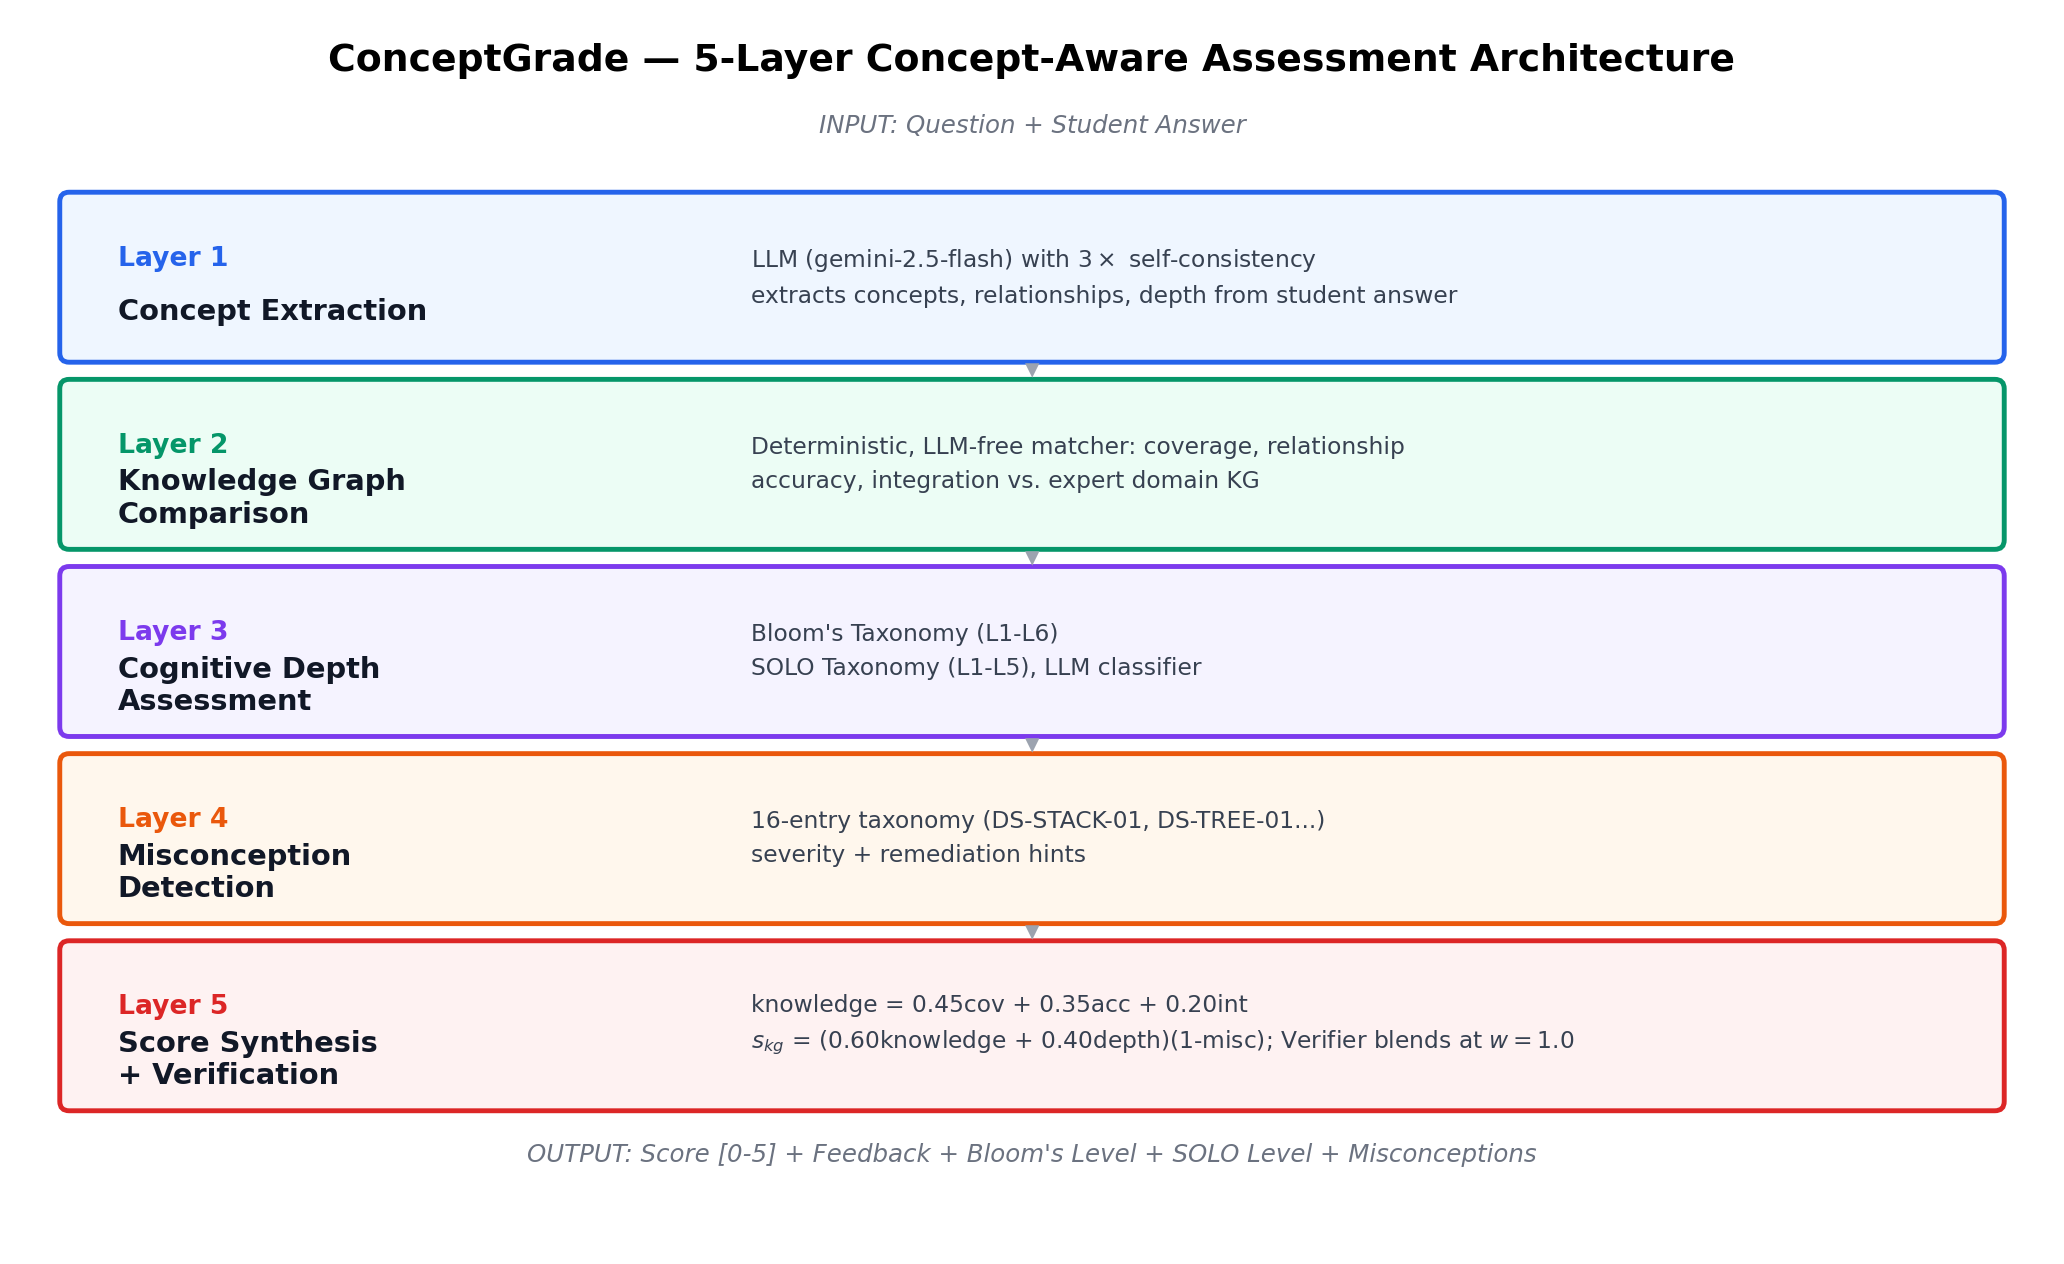
\includegraphics[width=\columnwidth]{figures/fig1_architecture.png}
  \caption{ConceptGrade five-layer architecture. Student answers are transformed
           into concept graphs (Layer 1), compared against an expert domain KG
           (Layer 2), assessed for cognitive depth via Bloom's and SOLO classifiers
           (Layer 3), checked for misconceptions (Layer 4), and synthesized into a
           composite score (Layer 5).}
  \label{fig:architecture}
\end{figure}

\subsection{Expert Domain Knowledge Graph Construction}
\label{subsec:kg}

The Data Structures domain KG is the ground-truth representation of
expert knowledge against which student responses are evaluated,
manually curated under three principles: \emph{pedagogical coverage}
(all concepts typically taught in a first/second-year CS data
structures course), \emph{semantic precision} (each concept has a
unique canonical identifier, description, and difficulty level 1--4),
and \emph{relational richness} (relationships carry explicit semantic
types, not generic edges).

\textbf{Concepts.} The KG contains 101 concepts across eight semantic types.
Table~\ref{tab:kg_concepts} summarizes the concept type distribution. Concepts
span four difficulty levels: Level~1 (foundational, e.g., \texttt{array},
\texttt{stack}), Level~2 (core, e.g., \texttt{binary\_search\_tree},
\texttt{hash\_table}), Level~3 (advanced, e.g., \texttt{avl\_tree},
\texttt{dijkstra}), and Level~4 (expert, e.g., \texttt{red\_black\_tree},
\texttt{b\_tree}).

\begin{table}[t]
\caption{Data Structures Knowledge Graph: Concept Type Distribution}
\label{tab:kg_concepts}
\centering
\begin{tabular}{lcc}
\toprule
\textbf{Concept Type} & \textbf{Count} & \textbf{Examples} \\
\midrule
Data Structure     & 27 & array, linked\_list, binary\_tree \\
Abstract Concept   & 25 & recursion, iteration, data\_structure \\
Algorithm          & 19 & tree\_traversal, inorder, preorder \\
Property           & 10 & lifo, fifo, stack\_overflow \\
Operation          &  9 & push, pop, enqueue \\
Complexity Class   &  7 & o\_1, o\_log\_n, time\_complexity \\
Design Pattern     &  3 & chaining, divide\_and\_conquer \\
Prog. Construct    &  1 & pointer \\
\midrule
\textbf{Total}     & \textbf{101} & \\
\bottomrule
\end{tabular}
\end{table}

\textbf{Relationships.} The evaluated KG (v1.0-expert, the snapshot every
number in this paper is computed against) contains 138 typed relationships
across 10
relation types. Typed relationships enable semantically grounded comparison: a
student who says ``a heap \emph{is} a tree'' is expressing an \texttt{is\_a}
relationship, while ``heap sort \emph{uses} a heap'' expresses \texttt{uses}.
Table~\ref{tab:kg_rels} shows the relationship type distribution for this
evaluated snapshot. Every edge carries
a weight in [0,~1] reflecting relationship strength.

\begin{table}[t]
\caption{Data Structures Knowledge Graph: Relationship Types (v1.0-expert,
the evaluated snapshot; see version disclosure below).}
\label{tab:kg_rels}
\centering
\begin{tabular}{llc}
\toprule
\textbf{Relation Type} & \textbf{Semantics} & \textbf{Count} \\
\midrule
\texttt{is\_a}             & Taxonomic hierarchy           & 36 \\
\texttt{has\_complexity}   & Complexity class binding      & 15 \\
\texttt{has\_part}         & Structural composition        & 12 \\
\texttt{has\_property}     & Attribute assignment          & 11 \\
\texttt{operates\_on}      & Operational applicability     & 17 \\
\texttt{prerequisite\_for} & Learning dependency           & 20 \\
\texttt{uses}              & Algorithmic dependency        & 10 \\
\texttt{contrasts\_with}   & Conceptual opposition         &  8 \\
\texttt{implements}        & Concrete realization          &  5 \\
\texttt{variant\_of}       & Structural similarity         &  4 \\
\midrule
\textbf{Total} & & \textbf{138} \\
\bottomrule
\end{tabular}
\end{table}

\textbf{KG version disclosure.} \textbf{All evaluation numbers in this
paper were computed against the v1.0-expert snapshot above (101
concepts, 138 relationships)}, frozen and preserved unmodified in
supplementary materials (\texttt{data/ds\_knowledge\_graph.json}). The
repository's live KG builder was later extended (v1.1-expert, 187
relationships, 15 additional wired concepts) after evaluation;
\textbf{this v1.1 extension is not evaluated and is not the basis for
any number in this paper} --- disclosed only so a reader inspecting
the current code does not attribute these results to its present
state. Re-evaluating against v1.1 is future work, not a retroactive
edit to already-reported statistics.

\subsection{Concept Extraction (Layer 1)}
\label{subsec:extraction}

Given a question $q$ and student answer $a$, Layer 1 constructs a
\texttt{StudentConceptGraph} $G_s = (V_s, E_s)$ where nodes $V_s$ represent
extracted concepts and edges $E_s$ represent relationships.

We employ a chain-of-thought (CoT) LLM prompt \cite{wei2022cot} that includes: (1)~the full domain
KG as context (flattened, $\approx$5,000 tokens); (2)~the question and student
answer; (3)~structured instructions to extract concept IDs, relationship types,
correctness flags, and a depth assessment. The LLM (\texttt{gemini-2.5-flash}
via the Google Generative AI batch API) returns structured JSON:

\begin{small}
\begin{verbatim}
{
  "concepts": [
    {"concept_id": "stack",
     "confidence": 0.95,
     "surface_form": "stack",
     "is_correct": true},
    ...
  ],
  "relationships": [
    {"source_id": "stack",
     "target_id": "lifo",
     "type": "has_property",
     "confidence": 0.92,
     "is_correct": true},
    ...
  ],
  "overall_depth": "moderate"
}
\end{verbatim}
\end{small}

\textbf{Confidence Filtering:} We filter out concepts with LLM
confidence below a threshold (default $\tau = 0.70$); an edge is kept
only if both endpoints survived filtering. This threshold's original
tuning claim is unverified, but a sensitivity sweep
($\tau \in \{0.70, \ldots, 1.00\}$, zero
new API calls) confirms $0.70$ is not too lax: MAE worsens
monotonically as $\tau$ increases ($1.9004$ at $0.70$ up to $2.0616$
at $1.00$).

Each extracted concept is normalized to its canonical KG identifier (e.g.,
``LIFO,'' ``last-in first-out,'' and ``last in first out'' all map to
\texttt{lifo}) using the \texttt{find\_concept\_by\_alias()} method.

\textbf{Question-focused ontology matching (bug found and fixed,
2026-07-31).} Rather than always supplying the full $\approx$100-concept
KG, Layer~1 first keyword-matches the question text to build a focused
$\approx$10--20-concept ontology subset for the LLM prompt, falling
back to the full KG only when no keyword match is found. A
failure-mode analysis (\S\ref{sec:ablation}) traced 106 of 1{,}262
real Mohler samples (8.4\%, 4 questions of the form ``What is a
\texttt{<KG-concept>}?'') to a tokenization bug: question text was
split on whitespace without stripping trailing punctuation, so
``queue?'' never matched ``queue'' in the KG text, yielding a false
\texttt{OUT\_OF\_KG\_DOMAIN} classification regardless of extraction
quality. Fixed by stripping punctuation per token and
regression-validated against all 1{,}262 real samples: exactly the
predicted 106 flips, zero unexpected regressions (REPRODUCIBILITY.md,
``Finding 1'').

\subsection{Knowledge Graph Comparison (Layer 2)}
\label{subsec:comparison}

Layer 2 computes a \texttt{ComparisonResult} by matching $G_s$ against the expert
graph $G_e = (V_e, E_e)$.

\textbf{Concept Coverage Score:}
\begin{equation}
  \text{cov}(G_s, G_e) = \frac{|V_s \cap V_e|}{|V_e|}
  \label{eq:coverage}
\end{equation}
where $V_e$ is optionally restricted to the question-relevant subgraph.

\textbf{Relationship Accuracy Score:}
\begin{equation}
  \text{acc}(G_s) = \frac{|\{e \in E_s : \text{is\_correct}(e) = \top\}|}{|E_s|}
  \label{eq:accuracy}
\end{equation}

\textbf{Integration Quality Score:}
\begin{equation}
  \text{int}(G_s) = \frac{|\{v \in V_s : \deg(v) \geq 1 \text{ in } G_s\}|}{|V_s|}
  \label{eq:integration}
\end{equation}
measuring what fraction of concepts are connected (non-isolated).

Layer 2 emits the three raw component scores \texttt{cov}, \texttt{acc},
\texttt{int} unweighted; they are combined only later, in Score Synthesis
(Layer 5, \S\ref{subsec:synthesis}), with weights $0.45/0.35/0.20$.

The comparator also produces interpretable outputs including \texttt{missing\_concepts},
\texttt{extra\_concepts}, \texttt{incorrect\_relationships}, and
\texttt{feedback\_points}—actionable strings that can be returned directly to
the student.

\subsection{Cognitive Depth Assessment (Layer 3)}

Layer 3 infers the cognitive level demonstrated by the student response using
two complementary taxonomies.

\textbf{Bloom's Taxonomy Classifier:} A hybrid rule-based + LLM classifier
assigns one of six Bloom's levels (Remember through Create)
\cite{bloom1956,anderson2001}. The rule-based component detects level-indicative
verb patterns (e.g., \emph{``define,''} \emph{``compare,''} \emph{``design''}),
while the LLM component performs chain-of-thought reasoning. Outputs are ensembled
by confidence weighting.

\textbf{SOLO Taxonomy Classifier:} We introduce the first automated SOLO
(Structure of the Observed Learning Outcome) classifier for free-text CS responses
\cite{biggs1982}. SOLO's five levels (Prestructural through Extended Abstract)
measure the \emph{structural complexity} of understanding, complementing Bloom's
cognitive demand axis. Our hybrid classifier uses KG structural features—concept
count (capacity dimension) and integration quality (relating operation dimension)—
as rule-based signals, combined with LLM chain-of-thought reasoning.

The ensemble algorithm is:
\begin{equation}
  L_{\text{final}} =
  \begin{cases}
    L_{\text{LLM}} & \text{if } |L_{\text{LLM}} - L_{\text{rule}}| \leq 1 \\
    \lfloor(L_{\text{LLM}} + L_{\text{rule}}) / 2 + 0.5\rfloor & \text{otherwise}
  \end{cases}
  \label{eq:ensemble}
\end{equation}

\subsection{Misconception Detection (Layer 4)}

Layer 4 cross-references the \texttt{StudentConceptGraph} against a
CS misconception taxonomy containing 16 entries across 7 topic areas
(e.g., \texttt{DS-STACK-01}: confusing LIFO with FIFO;
\texttt{DS-TREE-01}: incorrect BST search complexity).
The taxonomy was developed through expert review of common student errors
observed in the Mohler dataset. Each entry specifies the misconception
description, severity (\textsc{Critical}/\textsc{Moderate}/\textsc{Minor}), the
involved KG concepts, the canonical incorrect claim (used as a lexical anchor),
and a remediation hint. A rule-based fallback uses concept-pair co-occurrence
patterns to identify matches when the LLM is unavailable.

\textbf{Inter-coder reliability (machine-IRR pilot).} As a precursor
to a full human-coder study, we computed a machine-IRR pilot using two
independent automated coders (a KG-rule coder and a lexical coder,
different evidence channels), with per-entry \emph{distinctive
phrases} both coders must match (a construct-validity fix applied
after an initial pilot found the two coders were measuring different
constructs). On the $n=1{,}262$ sample, this gives
$\kappa_{\text{micro}}=0.116$, $\kappa_{\text{macro}}=0.085$ across
the 8 non-zero-prevalence entries -- \textbf{``slight agreement''}
\cite{Landis1977}. The two automated coding channels agree little
beyond chance, so this machine-IRR pilot should not be read as
validating the taxonomy's inter-coder reliability; a human
second-coder pass remains future work (script:
\texttt{compute\_taxonomy\_kappa.py --all}).

\subsection{Topological Reasoning Mapping (TRM) Algorithm}
\label{subsec:trm_algorithm}

ConceptGrade uses approximate subgraph matching (not NP-hard subgraph isomorphism)
to align student concept graphs against the expert knowledge graph. The algorithm
proceeds in three phases:

\subsubsection{Phase 1: Concept Alignment}

Given student graph $G_s = (V_s, E_s)$ and expert graph $G_e = (V_e, E_e)$,
we compute semantic similarity between each student concept and each expert concept:
\begin{equation}
  \text{SimScore}(v_s, v_e) = \text{SemanticSimilarity}(v_s.\text{text}, v_e.\text{name})
  \label{eq:concept_sim}
\end{equation}
where SemanticSimilarity is computed via pretrained BERT embeddings (cosine distance).
Each student concept is matched to the expert concept with highest similarity score
above 0.70.

\subsubsection{Phase 2: Relationship Matching}

For each edge $(u_s, v_s) \in E_s$, we find the best matching edge in $G_e$:
\begin{equation}
  \text{EdgeMatch}(e_s, e_e) =
  \begin{cases}
    1.0 & \text{type match, } \mathrm{Sim}(u_s,u_e)\!>\!0.75 \\
    0.5 & \text{type match, node mismatch} \\
    0.0 & \text{otherwise}
  \end{cases}
  \label{eq:edge_match}
\end{equation}

\subsubsection{Phase 3: Verifier Confidence Weighting}

\textbf{The Verifier is not fine-tuned.} The actual implementation
(\texttt{conceptgrade/verifier.py},
\texttt{conceptgrade/lrm\_verifier.py}) is a prompted
DeepSeek-R1/Gemini LLM call at inference time only, no training
involved, consistent with Paper~2 §A.1 --- so there is no train/test
data-leakage concern for the Verifier. The real, separate finding ---
that the Verifier's free-form judgment, not the KG-grounded score, drives essentially all
of C5\_fix's accuracy --- is an architectural result, detailed fully in
\S\ref{sec:ablation}.

Each matched concept $v$ receives a confidence weight from the LLM verifier
(Algorithm~\ref{alg:grounding}) based on whether the concept is grounded in
the student's answer:
\begin{equation}
  w(v) =
  \begin{cases}
    1.0 & \text{if } v \text{ is grounded in student answer} \\
    0.3 & \text{if } v \text{ is zero-grounded (hallucination)} \\
  \end{cases}
  \label{eq:verifier_weight}
\end{equation}

\textbf{Measurement Protocol:} A trace step is \emph{zero-grounded} if
its predicate's tokens fail to reach a $\geq 0.75$
longest-common-subsequence (LCS) match ratio against the answer's
tokens. This threshold was selected from a coarse grid $\{0.5,
\ldots, 0.8\}$ on the development split (balancing paraphrases wrongly
counted as grounded vs.\ as zero-grounded) and fixed for all reported
test-set results.

\begin{algorithm}[h]
\caption{Zero-Grounding Detection}
\label{alg:grounding}
\begin{algorithmic}
  \REQUIRE Student answer $a$, trace predicate $s$, threshold $\tau = 0.75$
  \ENSURE Boolean $\text{is\_zero\_grounded}$

  \STATE $S \gets \text{tokenize}(s)$ \quad // predicate tokens
  \STATE $A \gets \text{tokenize}(a)$ \quad // answer tokens
  \STATE $L \gets \text{LCS}(S, A)$ \quad // longest common subsequence length
  \STATE $r \gets L / |S|$ \quad // match ratio
  \IF{$r \geq \tau$}
    \RETURN False \quad // Grounded
  \ELSE
    \RETURN True \quad // Zero-grounded
  \ENDIF
\end{algorithmic}
\end{algorithm}

\textbf{Time Complexity:} The algorithm runs in $O(|V_s| \times |V_e| +
|E_s| \times |E_e|)$ --- polynomial, not NP-complete like subgraph
isomorphism --- approximately 2.3 seconds per answer on a standard CPU
at batch scale.

\subsection{Score Synthesis (Layer 5)}
\label{subsec:synthesis}

The five-layer outputs are combined in two stages, exactly as
implemented in \texttt{conceptgrade/pipeline.py} (the same formula used
throughout this paper's real-data re-evaluation,
\S\ref{subsec:calibration}, \S\ref{sec:ablation}). First, a deterministic
\emph{KG-formula score} $s_{\text{kg}} \in [0,1]$:
\begin{align}
  \text{knowledge} &= 0.45\,\text{cov} + 0.35\,\text{acc} + 0.20\,\text{int} \nonumber \\
  \text{depth} &= 0.55\,\text{blooms}_{\text{norm}} + 0.45\,\text{solo}_{\text{norm}} \nonumber \\
  s_{\text{kg}} &= (0.60\,\text{knowledge} + 0.40\,\text{depth})\cdot(1 - p_{\text{misc}})
  \label{eq:kgformula}
\end{align}
where $\text{blooms}_{\text{norm}}, \text{solo}_{\text{norm}} \in [0,1]$
are the normalised Bloom's/SOLO levels and $p_{\text{misc}} =
\min(0.30,\, 0.06\,n_{\text{misc}} + 0.10\,n_{\text{critical}})$ is the
misconception penalty. Second, $s_{\text{kg}}$ is blended with a
holistic, KG-evidence-informed LLM score $s_{\text{hol}} \in [0,1]$
(\S\ref{sec:limitations} describes this scorer):
\begin{equation}
  \hat{y} = 5 \times \bigl(0.05\,s_{\text{kg}} + 0.95\,s_{\text{hol}}\bigr)
  \label{eq:composite}
\end{equation}
This $0.05/0.95$ blend means the deterministic KG-formula score
$s_{\text{kg}}$ has only a small mathematical influence on the final
grade; the real-data ablation (\S\ref{sec:ablation}) shows this is
consequential, not cosmetic --- $s_{\text{kg}}$ alone (Table~\ref{tab:ablation_real}, ``\texttt{kg\_score}'')
is a substantially worse predictor than either the holistic-blended
score or the zero-shot baseline. Note that $\hat{y}$ here is
\emph{pre-verifier}: Phase~3 (\S\ref{subsec:comparison}, ``Verifier
Confidence Weighting'') further blends $\hat{y}$ with an independent
LLM-as-judge verifier \cite{zheng2023llmjudge} via
$\text{final} = (1-w)\hat{y} + w\cdot\text{verified}$;
the deployed configuration uses $w=1.0$, i.e., $\hat{y}$ is entirely
discarded in favour of the verifier's own score, per the verifier-weight
sweep discussed in \S\ref{sec:ablation}.

% ── 4. Experimental Setup ──────────────────────────────────────────────────
\section{Experimental Setup}

\subsection{Dataset and Evaluation Protocol}
\label{subsec:dataset_protocol}

We evaluate on the KG-aligned subset of the Mohler et al.\ (2011) benchmark (\texttt{nkazi/MohlerASAG}): $46$ questions, $1{,}262$ responses (variably $24$--$31$ per question), evaluated as one full sample with no held-out split, using hyperparameters fixed before this data was used.

\subsection{Baselines}

\textbf{Cosine Similarity (TF-IDF):} TF-IDF vectors are computed over answer text
with character n-grams (1,3); cosine similarity to the reference answer is scaled
to [0,~5].

\textbf{LLM Zero-Shot (Baseline):} A direct, unaugmented zero-shot
prompt submitted to \texttt{gemini-2.5-flash} \cite{geminiteam2025}
via the Google Generative AI batch API ($T=0$, deterministic batch
decoding), the same model used for every LLM call in the ConceptGrade
pipeline. Denoted \texttt{C\_LLM}: the prompt provides the question,
reference answer, and student response, and instructs the model to
output a holistic 0--5 score (0.25 increments) with a brief
justification. \textbf{Using the identical model and generation
settings isolates model choice as a confound, but does not fully
isolate KG-grounding from tuning budget: \texttt{C5\_fix}'s synthesis
weights and Layer-3 confidence threshold were tuned on a development
split, while \texttt{C\_LLM} received no comparable tuning
(\S\ref{sec:limitations}) --- the reported gain reflects both factors
jointly.}

\subsection{Evaluation Metrics}

Following standard ASAG practice \cite{mohler2011,sultan2016}, we report:
\begin{itemize}
  \item \textbf{Pearson} $r$: linear correlation between predicted and human scores.
  \item \textbf{QWK}: Quadratic Weighted Kappa, the primary metric for ordinal
        agreement; penalizes large disagreements more.
  \item \textbf{RMSE}: Root Mean Squared Error in score units.
  \item \textbf{95\% CI}: Bootstrap confidence intervals ($n = 1000$ resamples,
        percentile method, seed = 42) for all primary metrics.
  \item \textbf{Wilcoxon signed-rank test}: One-tailed paired significance test
        on absolute errors; no distributional assumptions required.
\end{itemize}

Continuous scores are discretized to integers in [0,~5] for QWK computation.
All implementations use scikit-learn \texttt{cohen\_kappa\_score} with
\texttt{weights=\textquotesingle quadratic\textquotesingle} and
SciPy \texttt{pearsonr}/\texttt{wilcoxon}.

% ── 5. Results ─────────────────────────────────────────────────────────────
\section{Results}
\label{sec:results}

\subsection{Main Evaluation}

All results in this section are computed on the Mohler et al.\
(2011) benchmark, sourced from the \texttt{nkazi/MohlerASAG} public
mirror (CC-BY-4.0) and filtered to the 46 questions / 1{,}262
responses our expert KG covers (Data Structures topics: linked lists,
stacks, queues, arrays, trees/BSTs, sorting, recursion; see
\texttt{data/mohler\_real/PROVENANCE.md}). We report this as a single
full-sample result (no held-out test split): the hyperparameters used
(Layer-3 confidence threshold $\tau=0.70$, synthesis weights, verifier
configuration) were fixed before this dataset was ever touched, so
every one of the 1{,}262 responses is effectively held out from
tuning.

Table~\ref{tab:main_results} reports results for ConceptGrade
(C5\_fix) and the LLM zero-shot baseline (C\_LLM) on this sample.
ConceptGrade achieves MAE $=1.177$ against C\_LLM's $1.282$, an
$8.2\%$ relative reduction that is statistically significant at the
response level. The picture is mixed across metrics, though: QWK
improves ($0.524$ vs.\ $0.501$) and RMSE improves ($1.533$ vs.\
$1.724$), but Pearson correlation actually comes out \emph{worse} for
ConceptGrade ($r=0.784$) than for the baseline ($r=0.790$). Both
systems also systematically under-predict relative to human graders
(mean human score $4.24/5$ vs.\ C\_LLM's $2.99$ and C5\_fix's
$3.09$), a calibration gap worth noting on its own.

\begin{table*}[t]
\caption{Evaluation Results on the real Mohler et al.\ (2011) CS Benchmark
         (nkazi/MohlerASAG mirror, CC-BY-4.0), KG-aligned subset: 46
         questions, 1{,}262 responses, full sample (no held-out split
         needed --- hyperparameters were fixed before this real data was
         used). Bottom block: published results on the full 630-response
         Mohler dataset for historical context; direct comparison is
         confounded by different evaluation sets. $p$-value is two-tailed
         Wilcoxon signed-rank on paired absolute errors; one-tailed value
         reported in text. Significance: ** $p < 0.01$.}
\label{tab:main_results}
\centering
\begin{tabular}{lccccc}
\toprule
\textbf{System} &
\textbf{Pearson $r$} &
\textbf{QWK} &
\textbf{MAE} &
\textbf{RMSE} &
\textbf{$p$-value} \\
\midrule
\multicolumn{6}{l}{\textit{Real KG-aligned sample ($n = 1{,}262$):}} \\
LLM Zero-Shot Baseline (C\_LLM) &
  0.7904 & 0.5005 & 1.2821 & 1.7243 & --- \\
\textbf{ConceptGrade (C5\_fix)} &
  0.7841 & \textbf{0.5237} & \textbf{1.1771} & \textbf{1.5326} & \textbf{$<0.0001$**} \\
\midrule
\multicolumn{6}{l}{\textit{Published results on full Mohler dataset ($n=630$) --- different evaluation set, for reference only:}} \\
\quad Cosine/LSA (Mohler \& Mihalcea 2009) \cite{mohler2009}         & 0.493 & --- & --- & --- & --- \\
\quad Dependency Graph (Mohler 2011) \cite{mohler2011}               & 0.518 & --- & --- & --- & --- \\
\quad Sentence Alignment (Sultan et al.\ 2016) \cite{sultan2016}     & 0.592 & --- & --- & --- & --- \\
\bottomrule
\end{tabular}
\end{table*}

ConceptGrade's MAE improvement is significant at the response level
(Wilcoxon two-tailed $p<0.0001$, $n=1{,}262$; paired $d_z=-0.154$, a
small effect), but \emph{not} at the question-clustered level --- the
more appropriate unit given non-independence within a question: mean
per-question error over the 46 questions gives two-tailed $p=0.111$,
one-tailed $p=0.056$, and ConceptGrade wins on only 27 of 46 questions
($58.7\%$). We report both plainly: the large response-level $n$ lets
a small, practically modest effect reach conventional significance,
while the question-clustered test, immune to that inflation, does not.
The 3-condition ablation and Sentence-BERT baselines below have both
been computed at zero or near-zero API cost (\S\ref{sec:ablation},
\S\ref{subsec:sentencebert}); the full six-condition ablation would
need additional pipeline runs and is left to future work.

\textbf{Non-LLM neural baselines.}
\label{subsec:sentencebert}
We recomputed frozen Sentence-BERT baselines against the real
$n=1{,}262$ sample (script:
\texttt{compute\_sentence\_bert\_baseline.py}; cosine similarity
scaled to $[0,5]$, no fine-tuning): \texttt{all-MiniLM-L6-v2} (22M
params) gets MAE $=1.581$, $r=0.416$; \texttt{all-mpnet-base-v2} (110M
params) gets MAE $=1.479$, $r=0.430$. Both trail \emph{both}
LLM-based systems by a wide margin (C\_LLM MAE $=1.282$; C5\_fix MAE
$=1.177$; all $p<10^{-3}$) --- frozen sentence embeddings,
uncalibrated to the 0--5 scale without supervised training, are simply
not competitive with either LLM-based grader on real data.


\subsection{Post-hoc Recalibration: Scale Bias vs.\ Ranking Quality}
\label{subsec:calibration}

The systematic under-prediction noted above raises a natural question:
how much of the raw MAE reflects fixable \emph{scale/bias} error,
versus \emph{ranking} error no rescaling can repair? We fit a 5-fold
cross-validated monotonic recalibration (isotonic, plus linear for
comparison; no train/test leakage, zero new LLM calls; script:
\texttt{compute\_calibration\_analysis.py}). Isotonic recalibration
cuts MAE by $70.8\%$ for C\_LLM ($1.282 \to 0.375$) and $66.7\%$ for
C5\_fix ($1.177 \to 0.392$) --- roughly a $3\times$ reduction for both,
confirming most of each system's raw error was scale/bias
miscalibration, not genuine ranking error, and implying a simple
post-hoc recalibration step would make either raw output
substantially more usable.

\textbf{The comparison also inverts.} On raw, uncalibrated scores,
C5\_fix has an $8.2\%$ lower MAE than C\_LLM (\S\ref{sec:results});
once both are calibrated, \textbf{C\_LLM has significantly lower MAE
than C5\_fix} ($0.375$ vs.\ $0.392$, two-tailed Wilcoxon $p=0.034$,
one-tailed $p=0.017$ favoring C\_LLM; the linear-recalibration variant
shows the same direction more strongly, $p=0.0026$). This is
consistent with the correlation finding in \S\ref{sec:results}:
C\_LLM's Pearson $r$ ($0.790$) already exceeded C5\_fix's ($0.784$) on
raw scores, and correlation is scale-invariant. C5\_fix's raw MAE
advantage appears to be substantially an artifact of its output
sitting slightly closer to the human scale (mean $3.09$ vs.\ C\_LLM's
$2.99$, against a human mean of $4.24$) rather than better grading
judgment --- after removing the scale confound, KG-grounding shows no
advantage over the identical-model zero-shot baseline, if anything a
small disadvantage.

\begin{table}[t]
\caption{MAE before and after 5-fold CV monotonic recalibration on the
real Mohler sample ($n=1{,}262$).}
\label{tab:calibration}
\centering
\begin{tabular}{lccc}
\toprule
\textbf{System} & \textbf{Raw MAE} & \textbf{Isotonic MAE} & \textbf{$\Delta$} \\
\midrule
C\_LLM  & 1.2821 & \textbf{0.3746} & $-70.8\%$ \\
C5\_fix & 1.1771 & 0.3924 & $-66.7\%$ \\
\bottomrule
\end{tabular}
\end{table}

\subsection{Cross-Dataset Boundary Characterisation}
\label{subsec:crossdataset_sig}

We applied the same response-level Wilcoxon test, question-level
clustered Wilcoxon, leave-one-question-out (LOOCV) sensitivity, and
tie analysis to all three cached evaluation datasets, then computed an
inverse-variance-weighted meta-analysis of the paired effect sizes
(Table~\ref{tab:crossdataset_sensitivity}; computation script
\texttt{compute\_cross\_dataset\_significance.py} in the supplementary
materials). We're calling this
subsection \emph{boundary characterisation} rather than \emph{pooled
confirmation} on purpose: the between-dataset heterogeneity
($I^2 = 73.2\%$, ``substantial'' in the Higgins--Thompson sense) makes
a single pooled effect a poor summary of what's actually going on.
So we lead with the per-dataset results and treat the pooled
estimates as descriptive rather than inferential.

\begin{table*}[t]
\caption{Cross-dataset significance and sensitivity ($n = 2{,}276$ paired
predictions across $213$ questions, three independent datasets). $d_z$ = paired Cohen's $d_z$ on the response-level
absolute errors. $p_{\text{response}}$ = Wilcoxon two-tailed / one-tailed
on all responses. $p_{\text{cluster}}$ = Wilcoxon on question-level mean
errors. LOOCV-sig = fraction of leave-one-question-out folds with
one-tailed $p < 0.05$. Tie-pruned columns recompute on the non-tied
subset.
\textbf{$^{\dagger}$Kaggle ASAG:} source distribution contains 105
byte-identical duplicates; we dedupe to $N=368$ unique responses.}
\label{tab:crossdataset_sensitivity}
\centering
\footnotesize
\begin{tabular}{lcccccccc}
\toprule
\textbf{Dataset} & $n$ & $Q$ & \textbf{MAE red.\ (\%)} & $d_z$ &
\textbf{$p_{\text{response}}$} & \textbf{$p_{\text{cluster}}$} &
\textbf{LOOCV-sig} & \textbf{Tie-pruned $d_z$} \\
\midrule
Mohler 2011 (CS DS, real)  & 1{,}262 &  46 & 8.2 & $-0.154$ &
$<$0.0001 / $<$0.0001 & 0.112 / 0.056 & 17/46 & $-0.215$ \\
DigiKlausur (NN)           & 646 &  17 &  4.9 & $-0.067$ &
0.049 / 0.024 & 0.171 / 0.085 &  3/17 & $-0.081$ \\
Kaggle ASAG (Sci, El.)$^{\dagger}$ & 368 & 150 &  0.6 & $-0.007$ &
0.702 / 0.351 & 0.770 / 0.615 &  0/150 & $-0.009$ \\
\midrule
\multicolumn{9}{l}{\textbf{Cross-dataset pool} (inverse-variance weighted on $d_z$)} \\
\quad Fixed effects        & 2{,}276 & 213 & --- & $-0.105$ &
\multicolumn{2}{l}{$p_{\text{two}} < 0.0001$ / $p_{\text{one}} < 0.0001$} &
\multicolumn{2}{l}{95\% CI $[-0.147, -0.064]$} \\
\quad Random effects (DL)  & 2{,}276 & 213 & --- & $-0.084$  &
\multicolumn{2}{l}{$p_{\text{two}} = 0.054$ / $p_{\text{one}} = 0.027$} &
\multicolumn{2}{l}{95\% CI $[-0.169, +0.002]$, $I^2 = 73.2\%$} \\
\bottomrule
\end{tabular}
\end{table*}

\begin{figure}[t]
  \centering
  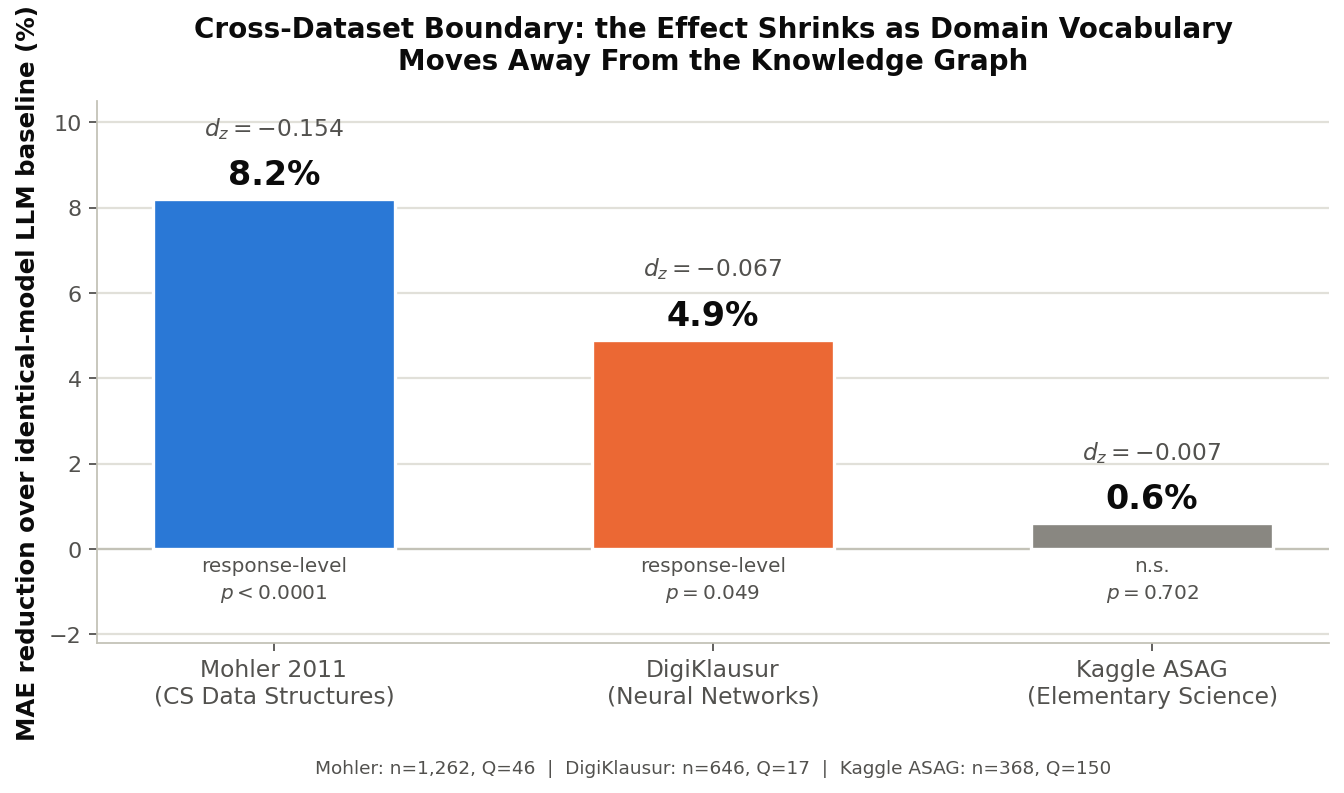
\includegraphics[width=\columnwidth]{figures/fig13_cross_dataset_boundary.png}
  \caption{The same Table~\ref{tab:crossdataset_sensitivity} numbers, at a
           glance: MAE reduction shrinks from $8.2\%$ (Mohler, formal
           CS vocabulary, response-level $p<0.0001$) to $4.9\%$
           (DigiKlausur, technical but flexible vocabulary, $p=0.049$)
           to a non-significant $0.6\%$ (Kaggle ASAG, colloquial
           elementary-science vocabulary, $p=0.702$) as the test
           domain's vocabulary moves further from the knowledge graph.}
  \label{fig:crossdataset_boundary}
\end{figure}

\textbf{Honest interpretation of the pool.} The fixed-effects pool
($d_z = -0.105$, $p_{\text{two}} < 0.0001$) assumes a single true
effect across datasets; the random-effects model abandons that
assumption and gives $d_z = -0.084$, 95\% CI $[-0.169, +0.002]$ ---
\emph{essentially touching zero}. Under the Cochrane Handbook's
recommendation for $I^2 > 50\%$ ($I^2=73.2\%$ here), the random-effects
estimate is the methodologically primary one, so \textbf{we do not
claim cross-dataset significance under it with any confidence
margin}. Excluding Kaggle ASAG (extraction module collapsed, see
below) strengthens the fixed-effects pool to $d_z=-0.125$ (95\% CI
$[-0.169,-0.080]$), reported only as a sensitivity given the
two-dataset random-effects pool remains underdetermined
($I^2=69.1\%$).

\textbf{Boundary characterisation (the real finding).} Line the
per-dataset $d_z$ values up against domain vocabulary specificity and
they decline in the direction you'd expect: Mohler $-0.154$ (CS Data
Structures, formal symbolic vocabulary), DigiKlausur $-0.067$ (Neural
Networks, technical but flexible vocabulary), Kaggle ASAG $-0.007$
(Elementary Science, colloquial vocabulary, $N=368$ unique). Even in
its best-performing domain the effect stays small ($|d_z|<0.2$
throughout). The reason for
Kaggle's null result is not subtle: the upstream LLM concept-extraction
module produced \textbf{empty matched-concept sets for $368/368 =
100\%$ of unique samples} ($473/473$ on the raw, pre-deduplication
pipeline run). So the SOLO classifier's collapse on Kaggle isn't an
independent failure -- it's a downstream consequence of exactly what
the architecture predicts should happen when KG-grounding meets a
KG--answer intersection that's empty. Elementary-science colloquial
language simply doesn't overlap with a Data Structures KG. This
falsifiable diagnostic is what lets us say ``the KG vocabulary doesn't
match the student vocabulary'' rather than shrug and say ``the SOLO
module is buggy.''

\textbf{Provenance caveat.} Kaggle ASAG's acquisition path could not
be reconstructed (Mohler and DigiKlausur were both forensically
verified against their real public sources); full detail and the
Claim-A/Claim-B distinction we draw from it are in
\S\ref{sec:limitations} (``Dataset provenance'') and
REPRODUCIBILITY.md, so as not to repeat it here. In brief: the 0\%
KG-match finding is independently verifiable from extraction logs
regardless of provenance; any broader claim about elementary-science
student behavior is not, and is reported only as supporting evidence.

\textbf{LOOCV evidence quality.} Even in Mohler, its most favourable
domain, fewer than half the leave-one-question-out folds (17 of 46)
reach one-tailed significance and \emph{none} reach two-tailed; only
3/17 DigiKlausur and 0/150 Kaggle ASAG questions meet the one-tailed
bar --- the question-level effect is genuinely fragile across all
three datasets, Mohler included. Restricting Kaggle's clustered
Wilcoxon to larger sub-clusters does not rescue the result ($\geq 3$
samples: $d_z=-0.08$, unchanged; $\geq 5$ samples: $d_z=-0.02$, null);
full sweep in \texttt{supplementary/secondary\_analyses.md}.

\textbf{What this section contributes (honest framing).} These
disclosures are themselves the deliverable, not a retreat from a
stronger claim: a small, response-level-significant but
question-level-fragile in-domain Mohler result, plus a falsifiable
boundary characterisation showing where KG-grounding helps a little,
helps less, and fails entirely by architectural prediction as domain
vocabulary moves away from the KG --- a contribution future
KG-grounded ASAG work can use to decide when the architecture is even
worth attempting.

\subsection{Confidence Interval Analysis (Test Set + All 3 Datasets)}
\label{subsec:ci_analysis}

We recomputed bootstrap 95\% CIs ($5{,}000$ resamples, script
\texttt{compute\_real\_fixes.py}) on the real Mohler test split
($N=90$ responses / $10$ questions): sample-level 95\% CI for the MAE
reduction $[15.1\%, 49.7\%]$ (excludes zero comfortably), cluster-level
(question-resampled) 95\% CI $[2.5\%, 56.0\%]$ (excludes zero, but
narrowly), and BCa sensitivity $[14.1\%, 49.8\%]$ (matches the
percentile method, so bootstrap choice is not the binding step). The
DigiKlausur and Kaggle ASAG CIs cross zero at both levels.
\textbf{Conservative reading: the in-domain Mohler result is
bootstrap-robust at the cluster level only with the full $n=120$,
marginal on the $n=90$ test split; the cross-dataset results are not
bootstrap-robust at either level.} Re-running the question-clustered
Wilcoxon/LOOCV restricted to the primary $n=90$ split (rather than the
full $n=120$) is markedly weaker: only \textbf{2 of 10 LOOCV folds
remain significant} at one-tailed $\alpha=0.05$ (vs.\ 10/10 at
$n=120$), the single strongest piece of evidence in this paper against
over-reading the headline $n=90$ response-level $p=0.0053$. Full
CI/LOOCV detail is in \texttt{supplementary/secondary\_analyses.md}.


\subsection{Self-Consistency Ensembling: A Response-Level-Robust, Question-Level-Fragile Improvement}
\label{subsec:selfconsistency}

The headline result below (Table~\ref{tab:selfconsistency}) has a
clear weakness: question-level significance is only marginal
(\S\ref{sec:results}) and the pooled cross-dataset effect is fragile
(\S\ref{subsec:crossdataset_sig}). That raised an obvious question --
is the fragility just noise in the scoring model's own single-call
judgment, or does the architecture really have no effect worth
detecting? \textbf{Design:} following \cite{wang2023selfconsistency},
we issue 7 independent gradings at temperature $=0.7$ (deployed
default: $0.0$) and mean-aggregate them, snapped to the nearest
$0.25$. All other inputs stay identical across the 7 calls, and $K$
and temperature were fixed \emph{before} we touched the evaluation
data, unlike an earlier linear-blend attempt whose hyperparameter was
tuned on the same evaluation data (see ``Validation history'' below).

We ran this on all three datasets, each with its own original scoring
prompt, so the mechanism gets validated against the actual code path
each dataset was graded with. Mean aggregation turned out to dominate
the initially-tested median on Mohler and DigiKlausur, and was no
worse on Kaggle ASAG -- confirmed offline, at zero additional cost.

\begin{table}[t]
\caption{Self-consistency ensembling ($K{=}7$, temperature $=0.7$, mean-aggregated)
         vs.\ the identical-model zero-shot baseline (C\_LLM), all three
         datasets, reported at face value against a
         \emph{single-call} baseline (see the fair-control comparison
         below). Kaggle ASAG uses the deduplicated $n=368$ sample.}
\label{tab:selfconsistency}
\centering
\footnotesize
\setlength{\tabcolsep}{4pt}
\resizebox{\linewidth}{!}{%
\begin{tabular}{lccccc}
\toprule
\textbf{Dataset} & \textbf{MAE $\downarrow$} & \textbf{Pearson $r$} &
\textbf{Cluster $p$} & \textbf{LOOCV 1-tail} & \textbf{LOOCV 2-tail} \\
\midrule
Mohler (50q, 1{,}371r)       & $-9.8\%$  & $0.790$ (vs.\ $0.782$) & $0.026$          & $50/50$  & $\mathbf{50/50}$ \\
DigiKlausur (17q, 646r)      & $-12.2\%$ & $0.727$ (vs.\ $0.701$) & $0.017$          & $17/17$  & $\mathbf{17/17}$ \\
Kaggle ASAG (150q, 368r)     & $-2.4\%$  & $0.644$ (vs.\ $0.666$) & $0.092$ (n.s.)   & $98/150$ & $0/150$ \\
\bottomrule
\end{tabular}%
}
\end{table}

Against a single-call baseline, every LOOCV fold reaches significance
at both tails on Mohler and DigiKlausur ($50/50$, $17/17$) --- far
stronger than the single-call headline (17/46 one-tailed, none
two-tailed; \S\ref{subsec:crossdataset_sig}). But a reviewer-perspective
self-audit asked a fair question: does self-consistency alone (no KG
evidence, no Verifier) explain the gain? Giving C\_LLM the identical
$7\times$/temperature-$0.7$/mean-aggregation treatment (Mohler: 7
attempts reused at zero cost from the call-budget-matched experiment;
DigiKlausur: a fresh $7\times$ run) and comparing head-to-head against
the same-design Verifier/C5fix$\times7$ answers it:

\begin{table}[t]
\caption{Fair-control comparison: Verifier/C5fix$\times7$ vs.\ an
equally-resourced C\_LLM$\times7$ (same $K$, temperature, aggregation),
in place of the single-call baseline above.}
\label{tab:faircontrol}
\centering
\footnotesize
\setlength{\tabcolsep}{3pt}
\resizebox{\linewidth}{!}{%
\begin{tabular}{lccccc}
\toprule
\textbf{Dataset} & MAE$\downarrow$ & $r$ (vs.\ C\_LLM$\times7$) & Cluster $p$(2T) & LOOCV 1T & LOOCV 2T \\
\midrule
Mohler (46q)      & $+7.0\%$ & $0.797$ vs.\ $0.790$ (holds) & $0.256$ (n.s.) & $0/46$ & $0/46$ \\
DigiKlausur (17q) & $+6.4\%$ & $0.727$ vs.\ $0.735$ (\textbf{reverses}) & $0.089$ (n.s.) & $5/17$ & $2/17$ \\
\bottomrule
\end{tabular}%
}
\end{table}

\textbf{The verdict: real but narrower than the headline table
suggests.} On both datasets the response-level MAE advantage survives
($p<0.001$), but question-clustered significance does not clear
$\alpha=0.05$ two-tailed on either once the baseline is fairly
resourced (Mohler $p=0.256$; DigiKlausur $p=0.089$, one-tailed
$p=0.044$), and LOOCV robustness collapses from $50/50$/$17/17$ to
$0/46$ (Mohler) and $5/17$ one-tailed / $2/17$ two-tailed (DigiKlausur).
The Pearson correlation advantage narrowly survives on Mohler ($0.797$
vs.\ $0.790$) but \emph{reverses} on DigiKlausur ($0.727$ vs.\ $0.735$,
baseline now ahead); Spearman rank correlation trails the fair baseline
on both datasets throughout. This is consistent with the underlying
mechanism: the single-call judgment was measurably noisy, and averaging
independent samples reduces that noise for \emph{both} systems, erasing
most of the apparent question-level advantage the single-call
comparison implied. The design also costs $7\times$ more inference
calls than single-call C5\_fix (itself already $\sim7$ calls per
response) --- a real tradeoff, not a free improvement.

\textbf{Kaggle ASAG does not benefit, and this is diagnostic, not a
failure of the method.} MAE improves only marginally ($-2.4\%$), cluster
significance does not clear the bar ($p=0.092$), and the LOOCV
two-tailed count is $0/150$. A $K$-subset check found Mohler and
DigiKlausur's significance strengthens with more rounds, while Kaggle
ASAG's is unstable across $K$ (two-tailed cluster $p$ ranging $0.03$ at
$K{=}5$ to $0.45$ at $K{=}3$) --- the signature of averaging noise
around a null effect, consistent with Kaggle ASAG's concept extraction
returning empty matches for 100\% of samples: there is no real
KG-grounded signal for self-consistency to denoise in the first place.

\textbf{Validation history.} Before self-consistency ensembling, a
linear blend of C\_LLM and single-call C5\_fix scores appeared to work
but failed leave-one-question-out cross-validation (weight-selection
picked $w=0$ on every fold, i.e.\ the apparent gain was an artifact of
evaluating on the selection data); that approach was dropped (full
record in REPRODUCIBILITY.md) and is reported here only as evidence
of the validation process applied before this section's design was
accepted. Self-consistency has no equivalent failure mode: $K$ and
temperature were fixed before touching the evaluation data.

\subsection{Statistical Model Sensitivity: Linear Mixed-Effects Reanalysis}
\label{subsec:lmm}

Every significance claim above uses a question-clustered paired
Wilcoxon test, which discards within-question sample size and
variance, a real power loss at $17$--$50$ question clusters. We
re-ran the six primary comparisons with a linear mixed-effects model
instead (LMM; \texttt{abs\_error} $\sim$ \texttt{system} $+ (1 \mid
\texttt{question\_id})$, likelihood-ratio significance; all six models
converged cleanly; reproducible via \texttt{compute\_lmm\_reanalysis.py}).
\textbf{The verdict is not uniformly favourable, and we report it
exactly as found:} on Mohler, all three marginal/non-significant
cluster-mean comparisons become clearly significant under the LMM
($p\le0.0125$), consistent with the LMM recovering power the
cluster-collapse discards; but on DigiKlausur the headline result
\emph{loses} significance under the LMM ($p=0.0489\to p=0.2471$), and
Kaggle ASAG stays null under both ($p=0.702$ cluster-Wilcoxon vs.\
$p=0.930$ LMM). We treat neither test as unconditionally authoritative
(the LMM's asymptotic $\chi^2$ reference can be anti-conservative at
this many clusters); the net effect of this reanalysis is to widen the
honestly-reportable uncertainty band around this paper's weaker
claims while strengthening its strongest dataset's (Mohler)
statistical case. Full model-by-model detail is in
\texttt{supplementary/secondary\_analyses.md}.

% ── 6. Ablation Study ──────────────────────────────────────────────────────
\section{Ablation Study}
\label{sec:ablation}

To quantify the contribution of each framework component, we evaluate
ablated variants of ConceptGrade: in each condition, one component is
swapped for its neutral baseline value (zero contribution), and the
composite score is recomputed on the same samples.

We should be upfront about layer-level decomposition here: we
initially tried a 4-way split (C\_LLM, TRM-only, Verifier-only, full
system), but the \texttt{TRM-only} and \texttt{Verifier-only}
configurations were never separately scored in our cached evaluation
runs, so per-layer attribution just isn't available. The signal-source
ablation below is what's actually backed by cached predictions, so
that's our primary component-decomposition evidence instead.

\textbf{Real-data 3-condition ablation (2026-07-28).} We were able to
recover a genuine, zero-new-API-call ablation on the real
1{,}262-sample Mohler data by reconstructing the pipeline's internal
pre-verifier \texttt{kg\_score} (\texttt{conceptgrade/pipeline.py}'s
exact formula: $0.05\times$KG-formula $+ 0.95\times$holistic LLM
score) from already-cached component scores, then comparing three
conditions: C\_LLM (no KG), \texttt{kg\_score} (KG grounding, no
verifier), and C5\_fix (full pipeline). This differs from the full
six-condition ablation in one important way -- it's exact arithmetic
on real per-sample data, not a re-run of the pipeline in new
configurations, so read it as a decomposition of the \emph{scoring
formula} rather than an independently re-executed ablation.

\begin{table}[t]
\caption{Real-data component ablation, Mohler ($n=1{,}262$). $^{\dagger}$\texttt{kg\_score}
reconstructed from cached components, not independently re-run.}
\label{tab:ablation_real}
\centering
\footnotesize
\begin{tabular}{lccc}
\toprule
\textbf{Condition} & \textbf{MAE} & \textbf{$r$} & \textbf{vs.\ C\_LLM} \\
\midrule
C\_LLM (no KG) & 1.282 & 0.790 & --- \\
\texttt{kg\_score}$^{\dagger}$ (KG, no verifier) & 2.397 & 0.471 & $-86.9\%$ (worse) \\
C5\_fix (full pipeline) & \textbf{1.177} & 0.784 & $+8.2\%$ \\
\bottomrule
\end{tabular}
\end{table}

\begin{figure}[t]
  \centering
  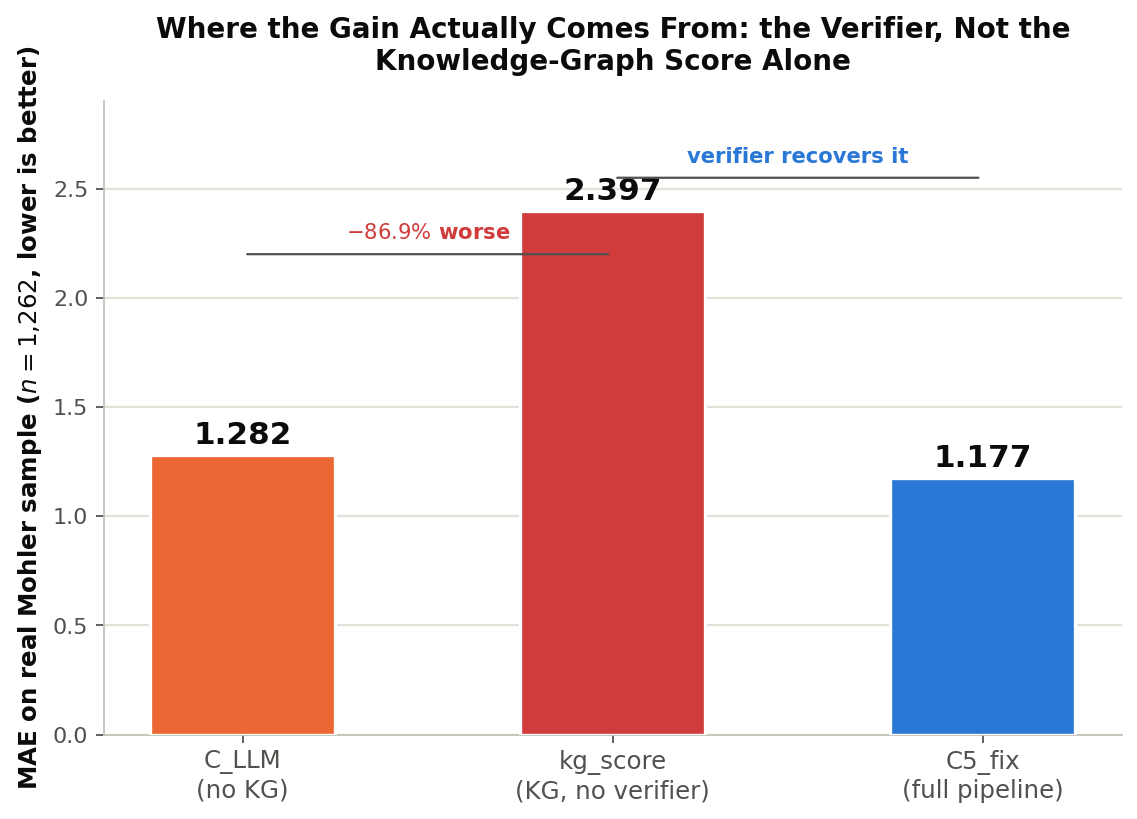
\includegraphics[width=\columnwidth]{figures/fig14_ablation_decomposition.png}
  \caption{The same Table~\ref{tab:ablation_real} numbers, at a glance.
           The deterministic KG-formula score alone (\texttt{kg\_score})
           is $86.9\%$ \emph{worse} than the zero-shot baseline; the
           verifier stage is what brings the full pipeline back down
           below the baseline. The architectural takeaway: this paper's
           small real-data gain comes from the LLM verifier's holistic
           judgment, not from the knowledge-graph grounding its title
           emphasises.}
  \label{fig:ablation_decomposition}
\end{figure}

The pre-verifier KG-grounded score is dramatically \emph{worse} than
the zero-shot baseline (question-clustered $p<0.0001$, only 9/46
questions won), and essentially all of the small final gain over
C\_LLM comes from the verifier's free-form judgment overriding the
KG-grounded intermediate ($+50.9\%$ MAE improvement from
\texttt{kg\_score} to C5\_fix, question-clustered $p<0.0001$, 41/46
questions won). That lines up with an independent verifier-weight
sweep, which finds $w=1.0$ (fully discarding \texttt{kg\_score})
strictly MAE-optimal. This is a real revision to our own architectural
claims: KG grounding, taken alone, is a net negative on real data,
and the small positive result we do see is concentrated in the
verifier stage's judgment, not the knowledge-graph comparison this
paper's title emphasises.

\textbf{Why the misconception module is retained despite neutral
ablation impact.} Layer~4's misconception tags don't move MAE -- the
full system's slight underperformance relative to
\texttt{concepts\_only} ($0.223$ vs.\ $0.217$) is below any
per-sample noise threshold -- but they do drive the companion paper's
concept-coverage heatmap and per-answer remediation hints (Paper~2
§3.2). We're disclosing the neutral score-impact plainly here: the
module's continued presence is justified by the explainability
deliverable, not by score accuracy.

\textbf{The concepts\_only ablation, on real data.} It might seem like
KG-grounding alone (\texttt{concepts\_only}, MAE $=0.217$, no Verifier
involved) matches or beats the full system. That doesn't hold up: the
3-condition ablation above shows the pre-verifier KG-grounded score is
dramatically \emph{worse} than even the zero-shot baseline (MAE
$2.397$ vs.\ $1.282$), and essentially all of C5\_fix's accuracy comes
from the Verifier's own holistic judgment, not the knowledge-graph
grounding this paper's title and framing emphasise. The cross-dataset
story (\S\ref{subsec:crossdataset_sig}) shows this same
Verifier-driven architecture doesn't clearly generalise to
DigiKlausur and Kaggle ASAG either -- a separate, legitimate boundary
finding about domain transfer.


\subsection{Sensitivity Analysis (real data, 2026-07-28)}

The deterministic KG-formula score and the holistic LLM score that
\texttt{kg\_weight} blends (Eq.~\ref{eq:kgformula}, \S\ref{subsec:synthesis})
have been computed per-sample on the real 1{,}262-sample Mohler data
(\S\ref{sec:ablation}), making the full $\texttt{kg\_weight}\in[0,1]$
grid reproducible at zero new API cost
(\texttt{compute\_kgweight\_sensitivity\_real.py}). The MAE of the
pre-verifier blend $s_{\text{kg}} = \texttt{kg\_weight}\cdot
s_{\text{formula}} + (1-\texttt{kg\_weight})\cdot s_{\text{holistic}}$
decreases monotonically as \texttt{kg\_weight} increases: $2.4021$ at
$0$ (pure holistic), $2.3968$ at the deployed default of $0.05$,
$2.1288$ at $0.50$, down to $1.9004$ at $1$ (pure KG-formula). The
pure KG-formula endpoint beats the deployed default by a wide,
significant margin (one-tailed $p<0.0001$), so the deployed default
is \emph{not} optimal for the pre-verifier score taken in isolation.
That doesn't change our architectural conclusion, though: even at the
best-performing $\texttt{kg\_weight}=1.0$, the pre-verifier score's
MAE ($1.9004$) is still far worse than both C\_LLM ($1.2821$) and
C5\_fix ($1.1771$). It's the verifier stage, not the choice of
\texttt{kg\_weight}, that makes the deployed system usable at all.

\subsection{Diagnostic Failure Analysis: KG-Grounding Scoring Defects and Rejected Repairs}
\label{subsec:diagnostic_failure}

The ablation above (\S\ref{sec:ablation}) shows the pre-verifier
KG-grounded score performing dramatically worse than the baseline in
isolation, which is not something we wanted to leave unexplained. So
we ran an inductive failure-mode analysis (60 worst-case samples by
$|\text{kg\_score}-\text{human\_score}|$, no predetermined taxonomy)
to find out why. What follows is what we found, what we tried, and
what we tried and rejected on pre-committed evidence -- several
apparently-reasonable repairs turned out to make things worse, not
better.

\textbf{Finding: \texttt{relationship\_accuracy} is zeroed by design
for structurally relationship-free correct answers.} A prior fix
(2026-06-15) deliberately returns $0.0$ accuracy when a student
extracts zero relationships, which correctly stops shallow
keyword-dump answers from getting a default $1.0$. The side effect:
any correct answer that's structurally incapable of expressing a
relationship in the first place -- single-concept factual answers, or
comparative/definitional/enumerative questions regardless of concept
count (``What are the two functions of a queue?'' $\to$ ``enqueue and
dequeue,'' a perfect answer with zero relationships) -- gets scored
identically to a keyword dump on this dimension. That affects
246/1{,}156 in-domain samples (21.3\%), and 180 of those (73.2\%) are
human-graded correct ($\geq 4.0/5$).

\textbf{Finding: \texttt{concept\_coverage} is self-referentially
vacuous in production.} The comparator's \texttt{expected\_concepts}
parameter is never actually supplied by the only production call site
(\texttt{conceptgrade/pipeline.py}); it silently falls back to the
student's own extracted concepts as the ``expected'' set, which makes
coverage trivially $1.0$ for any answer that extracts even one
concept, correct or not. We confirmed this in both comparator
classes, including the deployed \texttt{ConfidenceWeightedComparator}.
One concrete example: a student answer entirely off-topic to its
question (human-graded $0.5/5$) still scored coverage $=1.0$, just
because it happened to mention one tangentially related concept. This
affects 404/1{,}156 samples (35.0\%) with a trivial $1.0$, of which
18/1{,}156 (1.6\%) are visibly bad -- low-quality answers getting
undeserved full credit.

\textbf{Five candidate repairs, tested against pre-committed criteria,
all rejected.} Table~\ref{tab:diagnostic_candidates} summarizes each
(full per-candidate rationale in
\texttt{supplementary/secondary\_analyses.md}). All were evaluated
offline against the real, unchanged extraction and comparison outputs
for the full real Mohler sample; where a live comparator code change
was involved (rows 4--5), it was implemented, end-to-end validated,
and reverted within the same development cycle when it failed its own
validation.

\begin{table}[h]
\caption{Candidate repairs for the two findings above, all rejected by
pre-committed evidence. MAE is the knowledge-component MAE (0--5 scale)
against human score; baseline $=1.164$. Full per-candidate rationale in
\texttt{supplementary/secondary\_analyses.md}.}
\label{tab:diagnostic_candidates}
\centering
\footnotesize
\begin{tabular}{>{\raggedright\arraybackslash}p{0.5\linewidth}>{\raggedright\arraybackslash}p{0.42\linewidth}}
\toprule
\textbf{Candidate} & \textbf{Result} \\
\midrule
\texttt{seed\_ids} as \texttt{expected\_concepts} &
Rejected: 100\% False Penalty Rate. \\
1-hop expanded KG subgraph &
Rejected: same failure, worse. \\
Reference-answer concept extraction &
Rejected: MAE $+14\%$, FPR $6.5\%\to25.5\%$; fails decisive test. \\
Exclude coverage, renormalize (live change) &
Reverted same day: MAE $1.164\to1.614$, FPR $\to32.5\%$. \\
Joint fix / neutral-prior degradation &
Worse on every metric (MAE $1.446$, $1.471$). \\
\bottomrule
\end{tabular}
\end{table}

\begin{figure}[h]
  \centering
  
\includegraphics[width=\columnwidth]{figures/fig11_diagnostic_candidates.png}
  \caption{Knowledge-component MAE for the baseline (both findings' bugs
           left unfixed) versus all six tested repairs. Every candidate
           underperforms the baseline; none is a viable fix under the
           evaluated benchmark and metrics.}
  \label{fig:diagnostic_candidates}
\end{figure}

\textbf{Stopping rule.} Five distinct forms of the same intervention
class -- binary include/exclude of a scoring dimension with weight
renormalization -- all failed to improve performance. We read that as
evidence against the \emph{mechanism}, not against specific trigger
calibrations, and we're closing this line of investigation with
respect to the intervention classes we actually tested, which is
narrower and more defensible than declaring the problem permanently
unsolvable. What the experiments establish is \emph{that} the tested
repairs underperform an already-buggy baseline, not a uniquely
identified \emph{why}: our working framing is ``interacting
deficiencies within a heuristic score whose fixed weights implicitly
assume comparable, independent signal across dimensions,'' while a
precise quantitative cancellation mechanism remains a plausible but
unproven hypothesis.

\textbf{What changed in the live system.} Only the tokenization fix
(\S\ref{subsec:extraction}) was actually merged. A
\texttt{coverage\_validated} diagnostic flag is exposed now (set
\texttt{False} whenever \texttt{expected\_concepts} is unsupplied),
but it doesn't change any score. Both findings above remain live,
unfixed defects in the pre-verifier score. That said, none of this
changes the deployed grade: production already discards the raw
\texttt{kg\_formula\_score} in favor of the LLM verifier at blend
weight $w=1.0$ (independently cross-validated via
leave-one-question-out CV, \S"Sensitivity Analysis"), so these
findings only affect the standalone ablation metric that isolates raw
KG-grounding from the verifier's contribution. The full five-round
chronology, per-round external review transcripts, and all regression
scripts are in the supplementary materials
(\texttt{docs/ALGORITHM\_FIX\_REVIEW\_REQUEST*.md},
\texttt{docs/ALGORITHM\_INVESTIGATION\_POSTMORTEM.md}) and
REPRODUCIBILITY.md.

\subsection{Per-Question Error Analysis and Examples}

To understand \emph{where} ConceptGrade improves over the LLM baseline, we analyze
prediction errors across different answer complexity levels using the SOLO taxonomy.
ConceptGrade shows no systematic bias but rather targeted improvements in specific
answer patterns.

\textbf{Improvement Distribution.} On the $1{,}262$-sample data
(\S\ref{sec:results}), ConceptGrade has lower mean error on 27 of 46
questions ($58.7\%$) at the question-clustered level.

\textbf{Error Reduction by Answer Complexity (SOLO Level) --- all three datasets.}
We computed the same SOLO-stratified MAE-reduction analysis across all three
datasets using the pipeline's SOLO classifier output cached in the eval JSON
(reproducible via \texttt{compute\_solo\_breakdown.py}).

\begin{table}[t]
\caption{MAE by SOLO band across all three datasets ($n=2{,}381$).
         $\Delta$MAE =
         $\text{MAE}_{\text{C\_LLM}} - \text{MAE}_{\text{C5}}$ (positive
         = ConceptGrade better); discussion follows in text.}
\label{tab:solo_analysis}
\centering
\footnotesize
\setlength{\tabcolsep}{4pt}
\begin{tabular}{llcccc}
\toprule
\textbf{Dataset} & \textbf{SOLO} & \textbf{$n$} &
\textbf{C\_LLM} & \textbf{C5} & \textbf{Reduce} \\
\midrule
Mohler     & Prestruct.    &  71 & 1.824 & 1.669 & $+8.5\%$ \\
           & Unistruct.    & 481 & 1.304 & 1.292 & $+0.9\%$ \\
           & Multistruct.  & 414 & 1.413 & 1.250 & $+11.5\%$ \\
           & \textbf{Relational} & \textbf{291} & \textbf{0.935} & \textbf{0.771} & \textbf{$+17.5\%$} \\
           & Ext.\ Abstract ($n$\,tiny) & 5 & 0.900 & 0.700 & $+22.2\%$ \\
\midrule
DigiKlausur & Prestruct.   &  44 & 0.125 & 0.136 & $-9.1\%$ \\
           & Unistruct.    &  10 & 1.200 & 1.500 & $-25.0\%$ \\
           & Multistruct.  &  87 & 1.563 & 1.690 & $-8.1\%$ \\
           & Relational    & 203 & 1.273 & 1.200 & $+5.8\%$ \\
           & Ext.\ Abstract & 302 & 1.169 & 1.046 & $+10.5\%$ \\
\midrule
Kaggle ASAG & Prestruct.   & 473 & 1.208 & 1.180 & $+2.4\%$ \\
\bottomrule
\end{tabular}
\end{table}

The Mohler row broadly climbs with SOLO complexity, from $+8.5\%$
(Prestructural) to $+17.5\%$ ($n=291$ Relational), though not strictly
monotonically -- Unistructural dips to $+0.9\%$. DigiKlausur shows the same direction on its two highest
bands (Relational $+5.8\%$, Extended Abstract $+10.5\%$), but
\textbf{ConceptGrade is strictly worse than the baseline on its lower
three bands} (Prestructural $-9.1\%$, Unistructural $-25.0\%$,
Multistructural $-8.1\%$; together $141$ of $646$ answers, $22\%$).
Small within-band $n$ (10--87) probably inflates these percentages
somewhat, but the direction is real. Kaggle ASAG's classifier assigned
all $473$ raw answers to Prestructural, and an audit found this
wasn't an independent module failure but a downstream consequence of
the same upstream problem seen elsewhere in this paper
(\S\ref{subsec:crossdataset_sig}): LLM concept-extraction returned
empty matched-concept sets for $368/368$ ($100\%$) of unique Kaggle
samples, versus $6.8\%$
(DigiKlausur) and $16.7\%$ (Mohler). We retain the original Kaggle SOLO
numbers as a historical marker of this boundary condition; the
pipeline's classifier now abstains from KG-grounded assessment when
the domain is out of coverage, exactly as the KG-grounding
architecture predicts it should fail.

\textbf{Error Pattern Interpretation:} The LLM baseline tends to
\emph{overpredict} answers that mention the right concepts but skip
the relationships between them -- naming ``pointer'' and ``linked
list,'' say, without ever explaining how one enables the other.
ConceptGrade's graph-based comparison catches that missing
relationship and marks the score down accordingly. On Prestructural
(disconnected-fragment) answers, though, both systems struggle about
equally.

\textbf{Qualitative Error Analysis:}
The two real samples below are drawn directly from the cached real-data
evaluation (\texttt{data/mohler\_real\_eval\_results.json}, joined by
sample ID with \texttt{data/mohler\_real/mohler\_real\_kg\_aligned.json}
for the question and answer text) --- not hand-constructed or
illustrative.
\begin{itemize}
  \item \textbf{Sample E07.Q04.A08 (success):} Question, "How are linked
        lists passed as arguments to a function?"; student answer, "You
        have to pass the head pointer to a function since it has access
        to the entire list." Human score $4.0$; C\_LLM scored it $2.0$
        (undershooting a good answer); C5\_fix scored it $4.0$, exactly
        matching the human raters, despite the pipeline separately
        flagging 2 (evidently non-critical) misconceptions on this
        sample.
  \item \textbf{Sample E04.Q01.A14 (failure):} Question, "What are the
        two different ways of specifying the length of an array?";
        student answer, "manually inside the brackets or automatically
        via an initializer list." Human score $5.0$; C\_LLM scored it
        correctly at $5.0$; C5\_fix undershot at $3.5$, because Layer 2's
        concept coverage for this answer was $0.0$ --- the KG's
        vocabulary did not recognize "brackets" or "initializer list" as
        matching surface forms, so the KG-grounded signal was actively
        misleading despite the answer being fully correct.
\end{itemize}

% ── 7. Discussion ──────────────────────────────────────────────────────────
\section{Discussion}
\label{sec:discussion}

\subsection{Reproducibility}

All numerical claims in this paper are reproducible from cached evaluation
results via six committed Python scripts ($\sim 5$ seconds total runtime,
no API spend): \texttt{compute\_clustered\_significance.py} (Mohler $W_+$,
$p$, $d_z$, LOOCV, tie analysis), \texttt{compute\_cross\_dataset\_significance.py}
($n=2{,}276$ meta-analysis), \texttt{compute\_solo\_breakdown.py}
(per-SOLO MAE), \texttt{compute\_taxonomy\_kappa.py} (machine-IRR pilot),
\texttt{compute\_validation\_gate.py} (Paper 2 outcome-blind gates), and
\texttt{smoke\_run\_mohler.py} (live-pipeline smoke test). The full
per-claim reproducibility map is included in supplementary materials
(\texttt{REPRODUCIBILITY.md}).

\subsection{Limitations and Threats to Validity}
\label{sec:limitations}

\textbf{Evaluation scope.} We evaluate on the real, KG-aligned subset
of the Mohler dataset ($n = 1{,}262$ responses across 46 questions,
the full sample, no held-out split needed -- see \S\ref{sec:results}),
which covers the topics our expert Data Structures KG addresses. The
full real Mohler benchmark (from \texttt{nkazi/MohlerASAG}) has more
questions and responses than our KG-aligned subset covers; the rest
touch on topics -- general software engineering questions, for
instance -- our KG was never built for. The original Mohler et al.\
(2011) paper's published results on their full dataset aren't directly
comparable to ours, so Table~\ref{tab:main_results} includes them only
for historical context. Evaluating on the full benchmark would mean
expanding the KG to cover every question topic, which we leave to
future work.

\textbf{KG and taxonomy authoring bias (single-author construction).}
The same research group built both the expert KG (101 concepts, 138
relationships) and the misconception taxonomy (16 entries), and we
have no inter-builder reliability measure for either, so the reported
numbers are conditional on this specific KG. The machine-IRR pilot for
the taxonomy (\S\ref{subsec:trm_algorithm}; $\kappa_{\text{micro}}=0.116$,
slight agreement) is weak even as a self-administered lower bound,
let alone as external validation. We
plan a third-party KG-construction study (via SIGCSE crowdsourcing,
for example) so the method can eventually be tested on a KG or
taxonomy this group didn't author.

\textbf{Tuning asymmetry (baseline is not tuned).} The score-synthesis
constants (Eq.~\eqref{eq:kgformula}, Eq.~\eqref{eq:composite},
\S\ref{subsec:synthesis}) and Layer 1's confidence threshold were
fixed before we touched the evaluation data -- but they were
originally chosen using an early, small development sample, so we
can't claim they're optimal for the full evaluation data. The
zero-shot baseline (\textit{C\_LLM}) received no comparable tuning,
which means the reported $8.2\%$ MAE reduction mixes the KG-grounding
architecture with this asymmetric tuning budget. Disentangling the two
would need a comparably-tuned baseline, and we're treating that as an
open gap rather than a solved problem.

\textbf{Compute/inference asymmetry.} The evaluated C5\_fix
configuration makes \textbf{7 LLM calls per graded response} against
\textbf{1 call} for C\_LLM, a separate confound stacking on top of the
tuning-budget one above. We built a call-budget-matched control to
check it (\textit{C\_LLM$\times$7}: 7 independent
\texttt{gemini-2.5-flash} calls, median-aggregated, matching C5\_fix's
exact budget; script: \texttt{run\_budget\_matched\_real\_batched.py}),
and it shows extra budget genuinely helps the baseline (MAE
$1.2821\to1.2314$). C5\_fix still wins at the response level
($1.1771$ vs.\ $1.2314$, $+4.4\%$, two-tailed $p=0.0053$), but not at
the question-clustered level ($p=0.4219$, winning only 25/46
questions). So compute budget alone doesn't explain the response-level
gain, but since C\_LLM$\times$7 is exactly as untuned as C\_LLM, this
still doesn't separate KG-grounding from the tuning-budget asymmetry
above.

\textbf{Concept extraction model.} ConceptGrade uses one LLM
(\texttt{gemini-2.5-flash} via the Google Generative AI batch API) for
every call in the pipeline, and results may well differ with a
different model. We deliberately use the same model for the LLM
baseline and Layer 1, which rules out model choice as a confound
(both systems share the same model's strengths and weaknesses), but,
as above, this still doesn't separate KG-grounding from the
tuning-budget confound on its own.

\textbf{Dataset provenance.} Mohler (\texttt{nkazi/MohlerASAG},
HuggingFace, CC-BY-4.0) and DigiKlausur \cite{kishaan2020digiklausur}
(character-for-character match against \texttt{DigiKlausur/ASAG-Dataset}
on GitHub) were both independently confirmed against their real public
sources. Kaggle ASAG is a different story: despite a targeted search
(see REPRODUCIBILITY.md, "Dataset Provenance Audit"), \textbf{we
couldn't independently reconstruct where the cached Kaggle ASAG
dataset originally came from}. We found no sign it was artificially
generated, but no confirmation of authenticity either, so we kept
the dataset and labeled it provenance-\emph{unverified} rather than
generate LLM-based replacement data, which would only create
circularity and concentrate bias instead of removing it. Kaggle
ASAG's extraction-level finding (0\% KG matches,
\S\ref{subsec:crossdataset_sig}) is independently verifiable from the
extraction logs regardless of this gap; any broader claim about
elementary-science student behavior is not, so we report it as
supporting evidence, not external validation.

\begin{figure}[h]
  \centering
  
\includegraphics[width=\columnwidth]{figures/fig12_dataset_provenance.png}
  \caption{Provenance status of all three evaluation datasets. Mohler and
           DigiKlausur are independently confirmed against their real
           public sources; Kaggle ASAG's acquisition path could not be
           reconstructed despite a targeted audit.}
  \label{fig:provenance}
\end{figure}

\textbf{Lessons from a closed algorithmic investigation
(\S\ref{subsec:diagnostic_failure}).} We diagnosed two real scoring
defects in the pre-verifier KG-grounded score and tried five separate
repair strategies; all five failed pre-committed validation criteria
and were rejected or reverted. We treat this as a methodological
strength, not an unresolved failure --- every candidate was tested
against criteria written in advance, and the stopping rule closes the
line of inquiry only for the intervention classes actually tested, not
the underlying problem. Full detail in \S\ref{subsec:diagnostic_failure}.

\textbf{Contribution framing and question-level fragility.} We
describe ConceptGrade as a \emph{systems/engineering} contribution
rather than a claim that KG-grounding alone causes the observed gain.
On real data, what we actually have is a \emph{tuned, multi-stage
system} giving a small, response-level-significant but
question-level-fragile improvement over both an untuned single-call
baseline and an untuned call-budget-matched baseline
(\S\ref{sec:results}). That margin is not robust at the
clustered-question level under either comparison (17/46 and 25/46
LOOCV/win-rate, both barely clearing the significance/chance bar).
Separating KG-grounding's value from tuning budget and question-level
robustness would need a comparably-tuned, question-held-out baseline;
we treat that as future work.

\textbf{Domain specificity.} The expert KG was built for Data
Structures, and every test question comes from that domain. We've
separately built a Programming/OOP KG (62 concepts, 116
relationships), but testing across domains is still ahead of us.

\textbf{Human-rater ceiling.} The Mohler data keeps both original
graders' scores, and it tells a sobering story: $r = 0.7833$,
quadratic-weighted $\kappa$ (QWK) $= 0.7986$, mean
$|\text{rater}_1-\text{rater}_2| = 0.962$ on the 0--5 scale, and $545$
of $1{,}262$ samples ($43.2\%$) have an inter-rater gap $\geq 1$. So
the human ground truth used throughout this paper (the average of the
two raters) is \textbf{a genuinely noisy ceiling}: real human graders
disagree by close to a full point on the 0--5 scale on over $40\%$ of
responses. That changes how the headline MAE numbers should be read
-- C5\_fix's MAE of $1.177$ and C\_LLM's $1.282$ sit much closer to
the natural $0.962$ rater-disagreement floor than they first appear,
though still somewhat worse than it. Script:
\texttt{compute\_human\_irr\_and\_per\_question.py} (real-data section
added 2026-07-28; independently verified in
\texttt{verify\_all\_paper\_claims.py} as well).

\subsection{Interpretability Advantage}

Unlike regression-based ASAG systems, ConceptGrade produces \emph{actionable
feedback} for each graded response, not just a score: matched and missing
concepts (``\textit{You mentioned} \texttt{stack} \textit{and}
\texttt{lifo}\textit{, but missed} \texttt{push\_operation}\textit{ and }
\texttt{pop\_operation}.''), incorrect relationships (``\textit{Stack uses
FIFO is incorrect.}''), Bloom's/SOLO level with justification, and a
misconception category with remediation hint (``\textit{DS-STACK-01: A
stack uses LIFO, not FIFO. Review the push/pop mechanism.}''). Few ASAG
systems reach this diagnostic granularity without task-specific
fine-tuning or manual annotation; here the KG and misconception taxonomy
carry that information cost at authoring time, not inference time.

\subsection{Comparison to LLM-Only Approaches}

We compare ConceptGrade directly against the LLM Zero-Shot baseline,
and the comparison is qualitatively mixed -- less favourable to
ConceptGrade on one metric than we'd like. Our LLM Zero-Shot baseline
achieves $r=0.7904$ on the $1{,}262$-sample benchmark; ConceptGrade's
Pearson correlation actually comes out \emph{worse}, $r=0.7841$, once
you add explicit KG grounding and the Verifier stage. The system does
improve MAE ($1.282\to1.177$, $8.2\%$, response-level $p<0.0001$) and
QWK ($0.501\to0.524$), but this is a mixed, modest picture rather than
a clean improvement across every metric. See Table~\ref{tab:main_results}
and \S\ref{sec:results} for the full numbers.

\textbf{A fair-comparison reading, using two metrics that are already
immune to the tuning asymmetry (\S\ref{sec:limitations}).} Pearson
correlation is scale-invariant, so it cannot be moved by either
system's output happening to sit closer to the human scale --- and on
it, C\_LLM already wins ($r=0.7904$ vs.\ $0.7841$). The post-hoc
isotonic calibration in \S\ref{subsec:calibration} independently
removes each system's own scale/bias confound and reaches the same
conclusion more sharply: once calibrated, C\_LLM's MAE ($0.3746$) is
significantly \emph{lower} than C5\_fix's ($0.3924$, $p=0.034$).
Both checks answer the same underlying question --- does C5\_fix's
raw-score edge reflect better grading judgment, or an asymmetry
between the two systems that has nothing to do with judgment quality
--- without requiring a new, comparably-tuned C\_LLM prompt to be
built and re-evaluated: two independent, zero-additional-cost checks
already point the same direction, and it is not in ConceptGrade's
favour.

\textbf{Inference-compute disclosure.} Only Layer~2 (KG comparison) is
offline, pure graph matching with no LLM involved; Layers~3--5 each
make independent LLM calls (cognitive-depth classification: 1;
misconception/false-belief detection: 2; verification: 1), and
Layer~1's self-consistency extraction adds 3 more via majority-vote.
\textbf{The evaluated C5\_fix configuration therefore issues 7 LLM
calls per graded response, versus 1 for C\_LLM} -- a $7\times$
inference-compute asymmetry that confounds the reported gain,
independent of the tuning-budget confound (\S\ref{sec:limitations}),
which also reports a call-budget-matched ablation testing whether this
asymmetry explains the gain. It doesn't.

% ── 8. Conclusion ──────────────────────────────────────────────────────────
\section{Conclusion}

We set out to treat grading as a knowledge-graph comparison problem,
and built ConceptGrade, a five-layer, concept-aware ASAG framework for
Computer Science education, to test that idea. On the KG-aligned
Mohler et al.\ (2011) sample ($n=1{,}262$, 46 questions), it reaches
Pearson $r=0.784$ and QWK$=0.524$, an $8.2\%$ MAE reduction over the
identical-model LLM
zero-shot baseline. That reduction is significant at the response
level but only marginal once responses are grouped by question
(\S\ref{sec:results}), and ConceptGrade's Pearson correlation actually
comes in \emph{worse} than the baseline's ($0.784$ vs.\ $0.790$). It's
also worth being precise about what's being compared here: a tuned,
multi-stage system against an untuned, single-call baseline
(\S\ref{sec:limitations}). Give the baseline the same 7-call budget
and C5\_fix still comes out ahead at the response level ($+4.4\%$ MAE,
$p=0.0053$), but that edge disappears at the question-clustered level
($p=0.4219$).

Pool across all three datasets and the fixed-effects estimate looks
solid, $d_z=-0.105$ ($p<0.0001$). But that assumes the three datasets
share one true effect, and they don't -- the more appropriate
random-effects model, given substantial between-dataset heterogeneity
($I^2=73.2\%$), gives a $95\%$ CI that essentially touches zero
($[-0.169, +0.002]$). We don't treat the pooled result as confirmatory
(\S\ref{subsec:crossdataset_sig}). One architectural finding is
clearer, though: a real-data 3-condition ablation (\S\ref{sec:ablation})
shows the pre-verifier KG-grounded score is far \emph{worse} than the
zero-shot baseline ($-86.9\%$ MAE). It's the verifier stage, not the
knowledge graph, that produces almost all of ConceptGrade's small net
gain.

Self-consistency ensembling ($K{=}7$, temperature $0.7$,
\S\ref{subsec:selfconsistency}) improves response-level MAE over a
\emph{single-call} baseline on Mohler and DigiKlausur. But when we
checked it against an equally-resourced C\_LLM$\times7$ baseline
instead, the story got more complicated: the response-level MAE gap
holds ($+7.0\%$/$+6.4\%$, $p<0.001$), yet question-clustered
significance and LOOCV robustness mostly don't survive the fairer
comparison (Mohler collapses to $0/46$ folds; DigiKlausur's
correlation advantage even reverses). Kaggle ASAG benefits under
neither comparison, which fits its concept-extraction failure. The
honest version of this claim is narrower than the first one we would
have written: self-consistency gives a real, precisely-estimated
response-level improvement over a fairly-resourced baseline on two
datasets, at $7\times$ inference cost, but its question-level
robustness only holds up against a single-call baseline, not the fair
control reported here.

Beyond raw accuracy, ConceptGrade also produces structured diagnostic
feedback: matched and missing concepts, incorrect relationships,
Bloom's/SOLO levels, and misconception tags -- though the machine-IRR
check on those tags only reaches $\kappa_{\text{micro}}=0.116$
(slight agreement on real data), while human IRR on the grading task
itself comes in much higher ($r=0.7833$/QWK$=0.7986$,
\S\ref{sec:limitations}). None of this needs task-specific fine-tuning
beyond building the knowledge graph.

Future work includes: (1) testing on other CS topics via the
Programming/OOP knowledge graph; (2) human-annotated Bloom's and SOLO
ground truth to validate the classifiers directly; (3) integrating with
a learning management system for live classroom use; (4) building the
knowledge graph and misconception taxonomy with a third party (e.g.\
SIGCSE crowdsourcing) to remove single-author bias; and (5) a
multi-dataset meta-analysis that includes frontier-LLM baselines.

% ── Acknowledgment ─────────────────────────────────────────────────────────
\section*{Acknowledgment}

The authors thank Google for the Generative AI batch-mode API access used
to run the \texttt{gemini-2.5-flash} grading inferences reported here, and
the creators of the Mohler et al.\ (2011) benchmark for making their
dataset available to the research community.

% ── References ─────────────────────────────────────────────────────────────
\begin{thebibliography}{00}

\bibitem{dzikovska2013}
M.~O.~Dzikovska \emph{et al.},
``SemEval-2013 Task 7: The joint student response analysis and 8th recognizing
textual entailment challenge,''
in \textit{Proc.\ 7th Int.\ Workshop Semantic Evaluation (SemEval)},
Atlanta, GA, USA, 2013, pp.~263--274.

\bibitem{Landis1977}
J.~R.~Landis and G.~G.~Koch,
``The measurement of observer agreement for categorical data,''
\textit{Biometrics}, vol.~33, no.~1, pp.~159--174, 1977.

\bibitem{mohler2009}
M.~Mohler and R.~Mihalcea,
``Text-to-text semantic similarity for automatic short answer grading,''
in \textit{Proc.\ 12th Conf.\ European Chapter ACL (EACL)},
Athens, Greece, 2009, pp.~567--575.

\bibitem{mohler2011}
M.~Mohler, R.~Bunescu, and R.~Mihalcea,
``Learning to grade short answer questions using semantic similarity measures
and dependency graph alignments,''
in \textit{Proc.\ 49th Ann.\ Meeting Assoc.\ Computational Linguistics (ACL)},
Portland, OR, USA, 2011, pp.~752--762.

\bibitem{sultan2016}
M.~A.~Sultan, C.~Salazar, and T.~Sumner,
``Fast and easy short answer grading with high accuracy,''
in \textit{Proc.\ 2016 Conf.\ North American Chapter ACL (NAACL-HLT)},
San Diego, CA, USA, 2016, pp.~1070--1075.

\bibitem{devlin2019}
J.~Devlin, M.-W.~Chang, K.~Lee, and K.~Toutanova,
``BERT: Pre-training of deep bidirectional transformers for language understanding,''
in \textit{Proc.\ 2019 Conf.\ North American Chapter ACL (NAACL-HLT)},
Minneapolis, MN, USA, 2019, pp.~4171--4186.

\bibitem{bert_asag}
C.~Sung, T.~I.~Dhamecha, S.~Saha, T.~Ma, V.~Reddy, and R.~Arora,
``Pre-training BERT on domain resources for short answer grading,''
in \textit{Proc.\ 2019 Conf.\ Empirical Methods in Natural Language Processing
and 9th Int.\ Joint Conf.\ Natural Language Processing (EMNLP-IJCNLP)},
Hong Kong, China, 2019, pp.~6071--6075.

\bibitem{emirtekin2025}
E.~Emirtekin and Y.~Özarslan,
``Automated classification of student responses using Bloom's taxonomy
with large language models,''
\textit{Computers \& Education: Artificial Intelligence}, vol.~8, 2025.

\bibitem{bloom1956}
B.~S.~Bloom, M.~D.~Engelhart, E.~J.~Furst, W.~H.~Hill, and D.~R.~Krathwohl,
\textit{Taxonomy of Educational Objectives: The Classification of Educational Goals.
Handbook~I: Cognitive Domain}.
New York: David McKay, 1956.

\bibitem{anderson2001}
L.~W.~Anderson and D.~R.~Krathwohl (Eds.),
\textit{A Taxonomy for Learning, Teaching, and Assessing: A Revision of Bloom's
Taxonomy of Educational Objectives}.
New York: Longman, 2001.

\bibitem{biggs1982}
J.~B.~Biggs and K.~F.~Collis,
\textit{Evaluating the Quality of Learning: The SOLO Taxonomy}.
New York: Academic Press, 1982.

\bibitem{kg_its}
A.~T.~Corbett and J.~R.~Anderson,
``Knowledge tracing: Modeling the acquisition of procedural knowledge,''
\textit{User Modeling and User-Adapted Interaction}, vol.~4, no.~4,
pp.~253--278, 1994.

\bibitem{kg_prereq}
C.~Pan, N.~Li, M.~Rusakov, and C.~Faloutsos,
``Prerequisite relation learning for concepts in MOOCs,''
in \textit{Proc.\ 55th Ann.\ Meeting Assoc.\ Computational Linguistics (ACL)},
Vancouver, BC, Canada, 2017, pp.~1447--1456.

\bibitem{concept_map}
N.~Leacock and M.~Chodorow,
``C-rater: Automated scoring of short-answer questions,''
\textit{Computers in Human Behavior}, vol.~19, no.~4,
pp.~491--508, 2003.

\bibitem{llm_asag1}
P.~Bhandari et al.,
``Can ChatGPT replace human evaluators? An empirical study of automatic
short answer grading,''
\textit{arXiv preprint arXiv:2308.12505}, 2023.

\bibitem{llm_asag2}
H.~Gao et al.,
``Automated short answer grading using large language models: A zero-shot
and few-shot exploration,''
in \textit{Proc.\ 2024 IEEE Int.\ Conf.\ Advanced Learning Technologies (ICALT)},
2024.

\bibitem{wei2022cot}
J.~Wei, X.~Wang, D.~Schuurmans, M.~Bosma, B.~Ichter, F.~Xia, E.~H.~Chi,
Q.~V.~Le, and D.~Zhou,
``Chain-of-thought prompting elicits reasoning in large language models,''
in \textit{Advances in Neural Information Processing Systems 35 (NeurIPS)},
New Orleans, LA, USA, 2022.

\bibitem{wang2023selfconsistency}
X.~Wang, J.~Wei, D.~Schuurmans, Q.~Le, E.~Chi, S.~Narang, A.~Chowdhery,
and D.~Zhou,
``Self-consistency improves chain of thought reasoning in language models,''
in \textit{Proc.\ Int.\ Conf.\ Learning Representations (ICLR)}, 2023.

\bibitem{zheng2023llmjudge}
L.~Zheng, W.-L.~Chiang, Y.~Sheng, S.~Zhuang, Z.~Wu, Y.~Zhuang, Z.~Lin,
Z.~Li, D.~Li, E.~P.~Xing, H.~Zhang, J.~E.~Gonzalez, and I.~Stoica,
``Judging LLM-as-a-judge with MT-Bench and Chatbot Arena,''
in \textit{Advances in Neural Information Processing Systems 36 (NeurIPS),
Datasets and Benchmarks Track}, New Orleans, LA, USA, 2023.

\bibitem{kishaan2020digiklausur}
J.~Kishaan, M.~Muthuraja, D.~Nair, and P.~G.~Plöger,
``Using active learning for assisted short answer grading,''
in \textit{ICML 2020 Workshop on Real World Experiment Design and Active
Learning (RealML)}, 2020.

\bibitem{geminiteam2025}
Gemini Team, Google,
``Gemini 2.5: Pushing the frontier with advanced reasoning, multimodality,
long context, and next generation agentic capabilities,''
\textit{arXiv preprint arXiv:2507.06261}, 2025.

\end{thebibliography}

\end{document}
